\documentclass[twoside]{book}

% Packages required by doxygen
\usepackage{fixltx2e}
\usepackage{calc}
\usepackage{doxygen}
\usepackage[export]{adjustbox} % also loads graphicx
\usepackage{graphicx}
\usepackage[utf8]{inputenc}
\usepackage{makeidx}
\usepackage{multicol}
\usepackage{multirow}
\PassOptionsToPackage{warn}{textcomp}
\usepackage{textcomp}
\usepackage[nointegrals]{wasysym}
\usepackage[table]{xcolor}

% Font selection
\usepackage[T1]{fontenc}
\usepackage[scaled=.90]{helvet}
\usepackage{courier}
\usepackage{amssymb}
\usepackage{sectsty}
\renewcommand{\familydefault}{\sfdefault}
\allsectionsfont{%
  \fontseries{bc}\selectfont%
  \color{darkgray}%
}
\renewcommand{\DoxyLabelFont}{%
  \fontseries{bc}\selectfont%
  \color{darkgray}%
}
\newcommand{\+}{\discretionary{\mbox{\scriptsize$\hookleftarrow$}}{}{}}

% Page & text layout
\usepackage{geometry}
\geometry{%
  a4paper,%
  top=2.5cm,%
  bottom=2.5cm,%
  left=2.5cm,%
  right=2.5cm%
}
\tolerance=750
\hfuzz=15pt
\hbadness=750
\setlength{\emergencystretch}{15pt}
\setlength{\parindent}{0cm}
\setlength{\parskip}{3ex plus 2ex minus 2ex}
\makeatletter
\renewcommand{\paragraph}{%
  \@startsection{paragraph}{4}{0ex}{-1.0ex}{1.0ex}{%
    \normalfont\normalsize\bfseries\SS@parafont%
  }%
}
\renewcommand{\subparagraph}{%
  \@startsection{subparagraph}{5}{0ex}{-1.0ex}{1.0ex}{%
    \normalfont\normalsize\bfseries\SS@subparafont%
  }%
}
\makeatother

% Headers & footers
\usepackage{fancyhdr}
\pagestyle{fancyplain}
\fancyhead[LE]{\fancyplain{}{\bfseries\thepage}}
\fancyhead[CE]{\fancyplain{}{}}
\fancyhead[RE]{\fancyplain{}{\bfseries\leftmark}}
\fancyhead[LO]{\fancyplain{}{\bfseries\rightmark}}
\fancyhead[CO]{\fancyplain{}{}}
\fancyhead[RO]{\fancyplain{}{\bfseries\thepage}}
\fancyfoot[LE]{\fancyplain{}{}}
\fancyfoot[CE]{\fancyplain{}{}}
\fancyfoot[RE]{\fancyplain{}{\bfseries\scriptsize Generated by Doxygen }}
\fancyfoot[LO]{\fancyplain{}{\bfseries\scriptsize Generated by Doxygen }}
\fancyfoot[CO]{\fancyplain{}{}}
\fancyfoot[RO]{\fancyplain{}{}}
\renewcommand{\footrulewidth}{0.4pt}
\renewcommand{\chaptermark}[1]{%
  \markboth{#1}{}%
}
\renewcommand{\sectionmark}[1]{%
  \markright{\thesection\ #1}%
}

% Indices & bibliography
\usepackage{natbib}
\usepackage[titles]{tocloft}
\setcounter{tocdepth}{3}
\setcounter{secnumdepth}{5}
\makeindex

% Custom commands
\newcommand{\clearemptydoublepage}{%
  \newpage{\pagestyle{empty}\cleardoublepage}%
}

\usepackage{caption}
\captionsetup{labelsep=space,justification=centering,font={bf},singlelinecheck=off,skip=4pt,position=top}

%===== C O N T E N T S =====

\begin{document}

% Titlepage & ToC
\pagenumbering{alph}
\begin{titlepage}
\vspace*{7cm}
\begin{center}%
{\Large Ants\+\_\+\+And\+\_\+\+Doodlebugs }\\
\vspace*{1cm}
{\large Generated by Doxygen 1.8.13}\\
\end{center}
\end{titlepage}
\clearemptydoublepage
\pagenumbering{roman}
\tableofcontents
\clearemptydoublepage
\pagenumbering{arabic}

%--- Begin generated contents ---
\chapter{Hierarchical Index}
\section{Class Hierarchy}
This inheritance list is sorted roughly, but not completely, alphabetically\+:\begin{DoxyCompactList}
\item \contentsline{section}{Cell}{\pageref{classCell}}{}
\item \contentsline{section}{Grid}{\pageref{classGrid}}{}
\item \contentsline{section}{Organism}{\pageref{classOrganism}}{}
\begin{DoxyCompactList}
\item \contentsline{section}{Ant}{\pageref{classAnt}}{}
\item \contentsline{section}{Doodlebug}{\pageref{classDoodlebug}}{}
\end{DoxyCompactList}
\item \contentsline{section}{Production}{\pageref{classProduction}}{}
\item \contentsline{section}{Tests2}{\pageref{classTests2}}{}
\end{DoxyCompactList}

\chapter{Data Structure Index}
\section{Data Structures}
Here are the data structures with brief descriptions\+:\begin{DoxyCompactList}
\item\contentsline{section}{\textbf{ Ant} }{\pageref{classAnt}}{}
\item\contentsline{section}{\textbf{ Cell} }{\pageref{classCell}}{}
\item\contentsline{section}{\textbf{ Doodlebug} }{\pageref{classDoodlebug}}{}
\item\contentsline{section}{\textbf{ Grid} }{\pageref{classGrid}}{}
\item\contentsline{section}{\textbf{ Organism} }{\pageref{classOrganism}}{}
\item\contentsline{section}{\textbf{ Production} }{\pageref{classProduction}}{}
\item\contentsline{section}{\textbf{ Tests2} }{\pageref{classTests2}}{}
\end{DoxyCompactList}

\chapter{File Index}
\section{File List}
Here is a list of all files with brief descriptions\+:\begin{DoxyCompactList}
\item\contentsline{section}{\textbf{ Ant.\+cpp} }{\pageref{Ant_8cpp}}{}
\item\contentsline{section}{\textbf{ Ant.\+h} }{\pageref{Ant_8h}}{}
\item\contentsline{section}{\textbf{ Ants\+And\+Doodles.\+cpp} }{\pageref{AntsAndDoodles_8cpp}}{}
\item\contentsline{section}{\textbf{ Cell.\+cpp} }{\pageref{Cell_8cpp}}{}
\item\contentsline{section}{\textbf{ Cell.\+h} }{\pageref{Cell_8h}}{}
\item\contentsline{section}{\textbf{ Doodlebug.\+cpp} }{\pageref{Doodlebug_8cpp}}{}
\item\contentsline{section}{\textbf{ Doodlebug.\+h} }{\pageref{Doodlebug_8h}}{}
\item\contentsline{section}{\textbf{ Grid.\+cpp} }{\pageref{Grid_8cpp}}{}
\item\contentsline{section}{\textbf{ Grid.\+h} }{\pageref{Grid_8h}}{}
\item\contentsline{section}{\textbf{ Organism.\+cpp} }{\pageref{Organism_8cpp}}{}
\item\contentsline{section}{\textbf{ Organism.\+h} }{\pageref{Organism_8h}}{}
\item\contentsline{section}{\textbf{ Production.\+cpp} }{\pageref{Production_8cpp}}{}
\item\contentsline{section}{\textbf{ Production.\+h} }{\pageref{Production_8h}}{}
\item\contentsline{section}{\textbf{ Tests2.\+cpp} }{\pageref{Tests2_8cpp}}{}
\item\contentsline{section}{\textbf{ Tests2.\+h} }{\pageref{Tests2_8h}}{}
\end{DoxyCompactList}

\chapter{Data Structure Documentation}
\section{Ant Class Reference}
\label{classAnt}\index{Ant@{Ant}}


{\ttfamily \#include $<$Ant.\+h$>$}

Inheritance diagram for Ant\+:\begin{figure}[H]
\begin{center}
\leavevmode
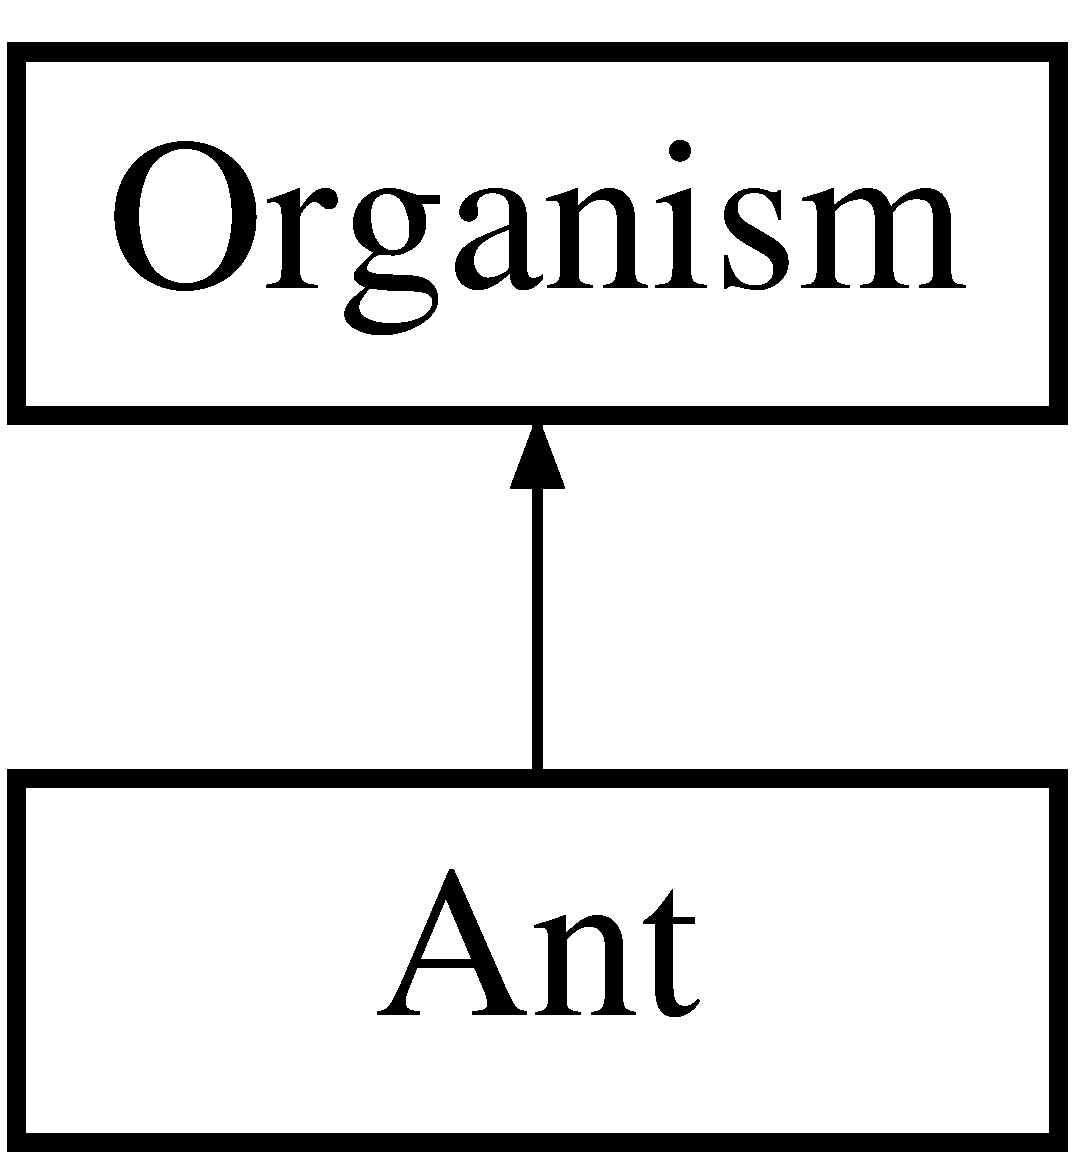
\includegraphics[height=2.000000cm]{classAnt}
\end{center}
\end{figure}
\subsection*{Public Member Functions}
\begin{DoxyCompactItemize}
\item 
\textbf{ Ant} (int r=0, int c=0, bool s=false)
\item 
bool \textbf{ move} (\textbf{ Grid} $\ast$g, int n)
\item 
bool \textbf{ breed} (\textbf{ Grid} $\ast$g, int n)
\item 
virtual \textbf{ $\sim$\+Ant} ()
\end{DoxyCompactItemize}
\subsection*{Additional Inherited Members}


\subsection{Constructor \& Destructor Documentation}
\mbox{\label{classAnt_ae4f5d63f7f1a820528ddd28b9913a284}} 
\index{Ant@{Ant}!Ant@{Ant}}
\index{Ant@{Ant}!Ant@{Ant}}
\subsubsection{Ant()}
{\footnotesize\ttfamily Ant\+::\+Ant (\begin{DoxyParamCaption}\item[{int}]{r = {\ttfamily 0},  }\item[{int}]{c = {\ttfamily 0},  }\item[{bool}]{s = {\ttfamily false} }\end{DoxyParamCaption})}

Constructs an \doxyref{Ant}{p.}{classAnt} and stores the given row and column. 
\begin{DoxyParams}{Parameters}
{\em r} & row to place \doxyref{Ant}{p.}{classAnt} \\
\hline
{\em c} & column to place \doxyref{Ant}{p.}{classAnt} \\
\hline
{\em s} & true if the \doxyref{Ant}{p.}{classAnt} should be skipped; false otherwise \\
\hline
\end{DoxyParams}


Referenced by breed().

\mbox{\label{classAnt_a33ca6bd592236726a18a2159908e4116}} 
\index{Ant@{Ant}!````~Ant@{$\sim$\+Ant}}
\index{````~Ant@{$\sim$\+Ant}!Ant@{Ant}}
\subsubsection{$\sim$\+Ant()}
{\footnotesize\ttfamily Ant\+::$\sim$\+Ant (\begin{DoxyParamCaption}{ }\end{DoxyParamCaption})\hspace{0.3cm}{\ttfamily [virtual]}}

Destructs an \doxyref{Ant}{p.}{classAnt}. Death of \doxyref{Ant}{p.}{classAnt} occurs when consumed by \doxyref{Doodlebug}{p.}{classDoodlebug}. 

\subsection{Member Function Documentation}
\mbox{\label{classAnt_af5d0af0b6e6be8526875773378627666}} 
\index{Ant@{Ant}!breed@{breed}}
\index{breed@{breed}!Ant@{Ant}}
\subsubsection{breed()}
{\footnotesize\ttfamily bool Ant\+::breed (\begin{DoxyParamCaption}\item[{\textbf{ Grid} $\ast$}]{g,  }\item[{int}]{n }\end{DoxyParamCaption})\hspace{0.3cm}{\ttfamily [virtual]}}

Gives birth to an \doxyref{Ant}{p.}{classAnt} in a randomly chosen empty adjacent cell. Can only give birth after surviving 3 steps. No birth occurs if all adjacent cells are occupied. Can give birth on next step if all adjacent cells are occupied. 
\begin{DoxyParams}{Parameters}
{\em g} & The grid with the organisms \\
\hline
{\em n} & The number of cells on an edge \\
\hline
\end{DoxyParams}
\begin{DoxyReturn}{Returns}
true if \doxyref{Ant}{p.}{classAnt} gave birth; false otherwise 
\end{DoxyReturn}


Implements \textbf{ Organism} \doxyref{}{p.}{classOrganism_a62e6c3a58974180f039c24889c5e6141}.



References ant, Ant(), Organism\+::col, down, left, Organism\+::orig\+Col, Organism\+::orig\+Row, right, Organism\+::row, Grid\+::set\+Cell\+Occupant(), stay, Organism\+::steps\+Since\+Breed, Organism\+::target\+Cell(), and up.



Referenced by Tests2\+::ants\+Breed\+Test(), and Production\+::one\+Ant\+Step().

\mbox{\label{classAnt_a2f7075f92830a8ce07f868c3feb68720}} 
\index{Ant@{Ant}!move@{move}}
\index{move@{move}!Ant@{Ant}}
\subsubsection{move()}
{\footnotesize\ttfamily bool Ant\+::move (\begin{DoxyParamCaption}\item[{\textbf{ Grid} $\ast$}]{g,  }\item[{int}]{n }\end{DoxyParamCaption})\hspace{0.3cm}{\ttfamily [virtual]}}

Checks if an adjacent cell is occupied, and if not, randomly selects one and moves to that cell. 
\begin{DoxyParams}{Parameters}
{\em g} & The grid with the organisms \\
\hline
{\em n} & The number of cells on an edge \\
\hline
\end{DoxyParams}
\begin{DoxyReturn}{Returns}
true if \doxyref{Ant}{p.}{classAnt} moved; false otherwise 
\end{DoxyReturn}


Implements \textbf{ Organism} \doxyref{}{p.}{classOrganism_a4d767696ff07b88656d35ceb3a0307e6}.



References ant, Organism\+::col, down, empty, left, Organism\+::orig\+Col, Organism\+::orig\+Row, right, Organism\+::row, Grid\+::set\+Cell\+Occupant(), Organism\+::skip, stay, Organism\+::steps\+Since\+Breed, Organism\+::target\+Cell(), and up.



Referenced by Tests2\+::ants\+Move\+Test(), and Production\+::one\+Ant\+Step().



The documentation for this class was generated from the following files\+:\begin{DoxyCompactItemize}
\item 
\textbf{ Ant.\+h}\item 
\textbf{ Ant.\+cpp}\end{DoxyCompactItemize}

\section{Cell Class Reference}
\label{classCell}\index{Cell@{Cell}}


{\ttfamily \#include $<$Cell.\+h$>$}

\subsection*{Public Member Functions}
\begin{DoxyCompactItemize}
\item 
\textbf{ Cell} ()
\item 
\textbf{ occupation\+Status} \textbf{ get\+Occupant} ()
\item 
void \textbf{ set\+Occupant} (\textbf{ occupation\+Status} g, \textbf{ Organism} $\ast$o\+\_\+ptr)
\item 
\textbf{ Organism} $\ast$ \textbf{ get\+Occupant\+Ptr} ()
\item 
virtual \textbf{ $\sim$\+Cell} ()
\end{DoxyCompactItemize}
\subsection*{Private Attributes}
\begin{DoxyCompactItemize}
\item 
\textbf{ Organism} $\ast$ \textbf{ org}
\item 
\textbf{ occupation\+Status} \textbf{ guest}
\end{DoxyCompactItemize}


\subsection{Constructor \& Destructor Documentation}
\mbox{\label{classCell_a394510643e8664cf12b5efaf5cb99f71}} 
\index{Cell@{Cell}!Cell@{Cell}}
\index{Cell@{Cell}!Cell@{Cell}}
\subsubsection{Cell()}
{\footnotesize\ttfamily Cell\+::\+Cell (\begin{DoxyParamCaption}{ }\end{DoxyParamCaption})}

Constructs a \doxyref{Cell}{p.}{classCell}. 

References empty, guest, and org.

\mbox{\label{classCell_a9fa559f7a28e2b4336c6879ca09304d8}} 
\index{Cell@{Cell}!````~Cell@{$\sim$\+Cell}}
\index{````~Cell@{$\sim$\+Cell}!Cell@{Cell}}
\subsubsection{$\sim$\+Cell()}
{\footnotesize\ttfamily Cell\+::$\sim$\+Cell (\begin{DoxyParamCaption}{ }\end{DoxyParamCaption})\hspace{0.3cm}{\ttfamily [virtual]}}

Destructs a \doxyref{Cell}{p.}{classCell}. 

Referenced by Tests2\+::get\+Occupant\+Ptr\+Test(), Tests2\+::set\+Cell\+Occupant\+Test(), Tests2\+::set\+Occupant\+Test(), and Grid\+::$\sim$\+Grid().



\subsection{Member Function Documentation}
\mbox{\label{classCell_a7dcb8bc75a2e2591b3fd52b5f7c28ab1}} 
\index{Cell@{Cell}!get\+Occupant@{get\+Occupant}}
\index{get\+Occupant@{get\+Occupant}!Cell@{Cell}}
\subsubsection{get\+Occupant()}
{\footnotesize\ttfamily \textbf{ occupation\+Status} Cell\+::get\+Occupant (\begin{DoxyParamCaption}{ }\end{DoxyParamCaption})}

Gets whether the cell is occupied by an \doxyref{Ant}{p.}{classAnt} or \doxyref{Doodlebug}{p.}{classDoodlebug}, or if it\textquotesingle{}s empty. \begin{DoxyReturn}{Returns}
the \doxyref{Ant}{p.}{classAnt} or \doxyref{Doodlebug}{p.}{classDoodlebug} in a cell. If not occupied, returns empty 
\end{DoxyReturn}


References guest.



Referenced by Grid\+::get\+Cell\+Occupant(), Tests2\+::get\+Occupant\+Test(), Tests2\+::set\+Cell\+Occupant\+Test(), and Tests2\+::set\+Occupant\+Test().

\mbox{\label{classCell_a00f1791893b97a29445e627c916e2a3f}} 
\index{Cell@{Cell}!get\+Occupant\+Ptr@{get\+Occupant\+Ptr}}
\index{get\+Occupant\+Ptr@{get\+Occupant\+Ptr}!Cell@{Cell}}
\subsubsection{get\+Occupant\+Ptr()}
{\footnotesize\ttfamily \textbf{ Organism} $\ast$ Cell\+::get\+Occupant\+Ptr (\begin{DoxyParamCaption}{ }\end{DoxyParamCaption})}

Gets the pointer in the \doxyref{Cell}{p.}{classCell}. \begin{DoxyReturn}{Returns}
The pointer to the \doxyref{Cell}{p.}{classCell} 
\end{DoxyReturn}


References org.



Referenced by Grid\+::get\+Cell\+Occupant\+Ptr(), and Tests2\+::get\+Occupant\+Ptr\+Test().

\mbox{\label{classCell_af205eff4eb59a50092f1661f02fcde15}} 
\index{Cell@{Cell}!set\+Occupant@{set\+Occupant}}
\index{set\+Occupant@{set\+Occupant}!Cell@{Cell}}
\subsubsection{set\+Occupant()}
{\footnotesize\ttfamily void Cell\+::set\+Occupant (\begin{DoxyParamCaption}\item[{\textbf{ occupation\+Status}}]{g,  }\item[{\textbf{ Organism} $\ast$}]{o\+\_\+ptr }\end{DoxyParamCaption})}

Sets the occupant of a \doxyref{Cell}{p.}{classCell}. 
\begin{DoxyParams}{Parameters}
{\em g} & ant, doodlebug, or empty \\
\hline
{\em o\+\_\+ptr} & the pointer to an organism or nullptr if empty \\
\hline
\end{DoxyParams}


References guest, and org.



Referenced by Tests2\+::get\+Occupant\+Ptr\+Test(), Tests2\+::get\+Occupant\+Test(), Grid\+::init\+Grid(), Grid\+::set\+Cell\+Occupant(), Tests2\+::set\+Cell\+Occupant\+Test(), and Tests2\+::set\+Occupant\+Test().



\subsection{Field Documentation}
\mbox{\label{classCell_aafc273a5125cf29742a8df6f5a5a881c}} 
\index{Cell@{Cell}!guest@{guest}}
\index{guest@{guest}!Cell@{Cell}}
\subsubsection{guest}
{\footnotesize\ttfamily \textbf{ occupation\+Status} Cell\+::guest\hspace{0.3cm}{\ttfamily [private]}}



Referenced by Cell(), get\+Occupant(), and set\+Occupant().

\mbox{\label{classCell_acbab180cc71423ae9ebe9c39ea4c8945}} 
\index{Cell@{Cell}!org@{org}}
\index{org@{org}!Cell@{Cell}}
\subsubsection{org}
{\footnotesize\ttfamily \textbf{ Organism}$\ast$ Cell\+::org\hspace{0.3cm}{\ttfamily [private]}}



Referenced by Cell(), get\+Occupant\+Ptr(), and set\+Occupant().



The documentation for this class was generated from the following files\+:\begin{DoxyCompactItemize}
\item 
\textbf{ Cell.\+h}\item 
\textbf{ Cell.\+cpp}\end{DoxyCompactItemize}

\section{Doodlebug Class Reference}
\label{classDoodlebug}\index{Doodlebug@{Doodlebug}}


{\ttfamily \#include $<$Doodlebug.\+h$>$}

Inheritance diagram for Doodlebug\+:\begin{figure}[H]
\begin{center}
\leavevmode
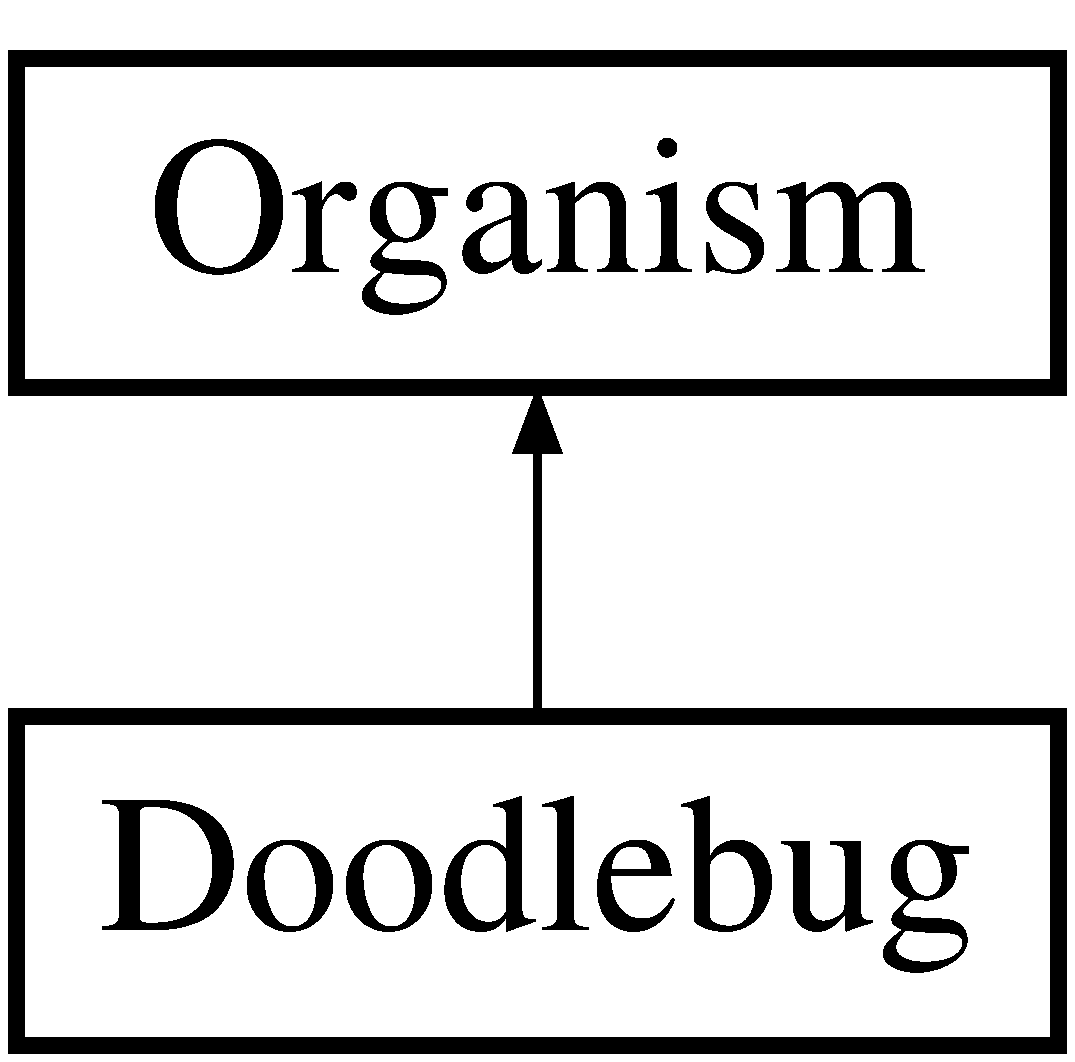
\includegraphics[height=2.000000cm]{classDoodlebug}
\end{center}
\end{figure}
\subsection*{Public Member Functions}
\begin{DoxyCompactItemize}
\item 
\textbf{ Doodlebug} (int r=0, int c=0, bool s=false)
\item 
int \textbf{ get\+Steps\+Since\+Ate} ()
\item 
bool \textbf{ move} (\textbf{ Grid} $\ast$g, int n)
\item 
bool \textbf{ breed} (\textbf{ Grid} $\ast$g, int n)
\item 
bool \textbf{ eat} (\textbf{ Grid} $\ast$g)
\item 
virtual \textbf{ $\sim$\+Doodlebug} ()
\end{DoxyCompactItemize}
\subsection*{Private Attributes}
\begin{DoxyCompactItemize}
\item 
int \textbf{ steps\+Since\+Ate}
\end{DoxyCompactItemize}
\subsection*{Additional Inherited Members}


\subsection{Constructor \& Destructor Documentation}
\mbox{\label{classDoodlebug_a09c1d55573a68f190e772a48c14f6b2b}} 
\index{Doodlebug@{Doodlebug}!Doodlebug@{Doodlebug}}
\index{Doodlebug@{Doodlebug}!Doodlebug@{Doodlebug}}
\subsubsection{Doodlebug()}
{\footnotesize\ttfamily Doodlebug\+::\+Doodlebug (\begin{DoxyParamCaption}\item[{int}]{r = {\ttfamily 0},  }\item[{int}]{c = {\ttfamily 0},  }\item[{bool}]{s = {\ttfamily false} }\end{DoxyParamCaption})}

\doxyref{Doodlebug}{p.}{classDoodlebug} Constructor. 
\begin{DoxyParams}{Parameters}
{\em r} & Row to initialize \doxyref{Doodlebug}{p.}{classDoodlebug} \\
\hline
{\em c} & Column to initialize \doxyref{Doodlebug}{p.}{classDoodlebug} \\
\hline
{\em s} & true if the \doxyref{Doodlebug}{p.}{classDoodlebug} should be skipped; false otherwise \\
\hline
\end{DoxyParams}


References steps\+Since\+Ate.



Referenced by breed().

\mbox{\label{classDoodlebug_ac318cc9acbd9a3af52348a236070d891}} 
\index{Doodlebug@{Doodlebug}!````~Doodlebug@{$\sim$\+Doodlebug}}
\index{````~Doodlebug@{$\sim$\+Doodlebug}!Doodlebug@{Doodlebug}}
\subsubsection{$\sim$\+Doodlebug()}
{\footnotesize\ttfamily Doodlebug\+::$\sim$\+Doodlebug (\begin{DoxyParamCaption}{ }\end{DoxyParamCaption})\hspace{0.3cm}{\ttfamily [virtual]}}

\doxyref{Doodlebug}{p.}{classDoodlebug} destructor. Death of \doxyref{Doodlebug}{p.}{classDoodlebug} occurs when \doxyref{Ant}{p.}{classAnt} not consumed in three steps. 

\subsection{Member Function Documentation}
\mbox{\label{classDoodlebug_a14e41f3251a7a092cec6943a5d7c976d}} 
\index{Doodlebug@{Doodlebug}!breed@{breed}}
\index{breed@{breed}!Doodlebug@{Doodlebug}}
\subsubsection{breed()}
{\footnotesize\ttfamily bool Doodlebug\+::breed (\begin{DoxyParamCaption}\item[{\textbf{ Grid} $\ast$}]{g,  }\item[{int}]{n }\end{DoxyParamCaption})\hspace{0.3cm}{\ttfamily [virtual]}}

Gives birth to a \doxyref{Doodlebug}{p.}{classDoodlebug} in an adjacent cell. Can only give birth after surviving for eight steps. Doesn\textquotesingle{}t give birth if adjacent cells occupied. Can give birth on next step if all adjacent cells are occupied. 
\begin{DoxyParams}{Parameters}
{\em g} & The grid containing the organisms \\
\hline
{\em n} & The number of cells along an edge of the grid \\
\hline
\end{DoxyParams}
\begin{DoxyReturn}{Returns}
true if birth given; false otherwise 
\end{DoxyReturn}


Implements \textbf{ Organism} \doxyref{}{p.}{classOrganism_a62e6c3a58974180f039c24889c5e6141}.



References Organism\+::col, doodlebug, Doodlebug(), down, left, Organism\+::orig\+Col, Organism\+::orig\+Row, right, Organism\+::row, Grid\+::set\+Cell\+Occupant(), stay, Organism\+::steps\+Since\+Breed, Organism\+::target\+Cell(), and up.



Referenced by Tests2\+::doodle\+Breed\+Test(), and Production\+::one\+Doodlebug\+Step().

\mbox{\label{classDoodlebug_a4ed23795ee677ac6f87c5d01911560f4}} 
\index{Doodlebug@{Doodlebug}!eat@{eat}}
\index{eat@{eat}!Doodlebug@{Doodlebug}}
\subsubsection{eat()}
{\footnotesize\ttfamily bool Doodlebug\+::eat (\begin{DoxyParamCaption}\item[{\textbf{ Grid} $\ast$}]{g }\end{DoxyParamCaption})}

Eats an \doxyref{Ant}{p.}{classAnt} in an adjacent cell. \begin{DoxyReturn}{Returns}
true if \doxyref{Ant}{p.}{classAnt} eaten; false otherwise 
\end{DoxyReturn}


References Organism\+::col, empty, Grid\+::get\+Cell\+Occupant(), Grid\+::get\+Cell\+Occupant\+Ptr(), Organism\+::row, and steps\+Since\+Ate.



Referenced by move().

\mbox{\label{classDoodlebug_a7b27c25112ca7594c456fdf944338d82}} 
\index{Doodlebug@{Doodlebug}!get\+Steps\+Since\+Ate@{get\+Steps\+Since\+Ate}}
\index{get\+Steps\+Since\+Ate@{get\+Steps\+Since\+Ate}!Doodlebug@{Doodlebug}}
\subsubsection{get\+Steps\+Since\+Ate()}
{\footnotesize\ttfamily int Doodlebug\+::get\+Steps\+Since\+Ate (\begin{DoxyParamCaption}{ }\end{DoxyParamCaption})}

Gets number of steps since the \doxyref{Doodlebug}{p.}{classDoodlebug} ate. \begin{DoxyReturn}{Returns}
number of steps since the \doxyref{Doodlebug}{p.}{classDoodlebug} ate 
\end{DoxyReturn}


References steps\+Since\+Ate.



Referenced by Tests2\+::get\+Steps\+Since\+Ate\+Test(), and Production\+::one\+Doodlebug\+Step().

\mbox{\label{classDoodlebug_afb9e8b67fd66543f664b855f30546f2e}} 
\index{Doodlebug@{Doodlebug}!move@{move}}
\index{move@{move}!Doodlebug@{Doodlebug}}
\subsubsection{move()}
{\footnotesize\ttfamily bool Doodlebug\+::move (\begin{DoxyParamCaption}\item[{\textbf{ Grid} $\ast$}]{g,  }\item[{int}]{n }\end{DoxyParamCaption})\hspace{0.3cm}{\ttfamily [virtual]}}

Moves the \doxyref{Doodlebug}{p.}{classDoodlebug} to an adjacent cell. Does not move if other Doodlebugs are occuping adjacent cells. 
\begin{DoxyParams}{Parameters}
{\em g} & The grid containing the organisms \\
\hline
{\em n} & The number of cells along an edge of the grid \\
\hline
\end{DoxyParams}
\begin{DoxyReturn}{Returns}
true if moved; false otherwise 
\end{DoxyReturn}


Implements \textbf{ Organism} \doxyref{}{p.}{classOrganism_a4d767696ff07b88656d35ceb3a0307e6}.



References ant, Organism\+::col, doodlebug, down, eat(), empty, Grid\+::get\+Cell\+Occupant(), left, Organism\+::orig\+Col, Organism\+::orig\+Row, right, Organism\+::row, Grid\+::set\+Cell\+Occupant(), Organism\+::skip, stay, steps\+Since\+Ate, Organism\+::steps\+Since\+Breed, Organism\+::target\+Cell(), and up.



Referenced by Tests2\+::doodle\+Move\+Test(), and Production\+::one\+Doodlebug\+Step().



\subsection{Field Documentation}
\mbox{\label{classDoodlebug_ac810c36d96a08bff696909ff2495a120}} 
\index{Doodlebug@{Doodlebug}!steps\+Since\+Ate@{steps\+Since\+Ate}}
\index{steps\+Since\+Ate@{steps\+Since\+Ate}!Doodlebug@{Doodlebug}}
\subsubsection{steps\+Since\+Ate}
{\footnotesize\ttfamily int Doodlebug\+::steps\+Since\+Ate\hspace{0.3cm}{\ttfamily [private]}}



Referenced by Doodlebug(), eat(), get\+Steps\+Since\+Ate(), and move().



The documentation for this class was generated from the following files\+:\begin{DoxyCompactItemize}
\item 
\textbf{ Doodlebug.\+h}\item 
\textbf{ Doodlebug.\+cpp}\end{DoxyCompactItemize}

\section{Grid Class Reference}
\label{classGrid}\index{Grid@{Grid}}


{\ttfamily \#include $<$Grid.\+h$>$}

\subsection*{Public Member Functions}
\begin{DoxyCompactItemize}
\item 
\textbf{ Grid} (int n\+Squares\+On\+A\+Side=20)
\item 
\textbf{ occupation\+Status} \textbf{ get\+Cell\+Occupant} (int r, int c)
\item 
void \textbf{ set\+Cell\+Occupant} (int r, int c, \textbf{ occupation\+Status} g, \textbf{ Organism} $\ast$o\+\_\+ptr)
\item 
\textbf{ Organism} $\ast$ \textbf{ get\+Cell\+Occupant\+Ptr} (int r, int c)
\item 
void \textbf{ init\+Grid} (int grid\+Size, int num\+Ants, int num\+Doodlebugs)
\item 
void \textbf{ print\+Grid} ()
\item 
virtual \textbf{ $\sim$\+Grid} ()
\end{DoxyCompactItemize}
\subsection*{Private Attributes}
\begin{DoxyCompactItemize}
\item 
int \textbf{ n}
\item 
\textbf{ Cell} $\ast$$\ast$ \textbf{ cell\+Arr\+Ptr}
\end{DoxyCompactItemize}


\subsection{Constructor \& Destructor Documentation}
\mbox{\label{classGrid_adcbfe5deb09aefc90ffe7b54762ea197}} 
\index{Grid@{Grid}!Grid@{Grid}}
\index{Grid@{Grid}!Grid@{Grid}}
\subsubsection{Grid()}
{\footnotesize\ttfamily Grid\+::\+Grid (\begin{DoxyParamCaption}\item[{int}]{n\+Squares\+On\+A\+Side = {\ttfamily 20} }\end{DoxyParamCaption})}

\doxyref{Grid}{p.}{classGrid} Constructor. 
\begin{DoxyParams}{Parameters}
{\em n\+Squares\+On\+A\+Side} & Number of squares on a side of the board \\
\hline
\end{DoxyParams}


References cell\+Arr\+Ptr, and n.

\mbox{\label{classGrid_a3661d0a7f998caaaf8627d7a67072116}} 
\index{Grid@{Grid}!````~Grid@{$\sim$\+Grid}}
\index{````~Grid@{$\sim$\+Grid}!Grid@{Grid}}
\subsubsection{$\sim$\+Grid()}
{\footnotesize\ttfamily Grid\+::$\sim$\+Grid (\begin{DoxyParamCaption}{ }\end{DoxyParamCaption})\hspace{0.3cm}{\ttfamily [virtual]}}

Destructs a \doxyref{Grid}{p.}{classGrid}. 

References cell\+Arr\+Ptr, n, and Cell\+::$\sim$\+Cell().



Referenced by Tests2\+::doodle\+Eat\+Test(), Tests2\+::get\+Cell\+Occupant\+Ptr\+Test(), Tests2\+::get\+Cell\+Occupant\+Test(), Tests2\+::get\+Steps\+Since\+Ate\+Test(), Tests2\+::get\+Steps\+Since\+Breed\+Test(), Tests2\+::grid\+Test(), Tests2\+::init\+Grid\+Test(), Tests2\+::one\+Ant\+Step\+Test(), Tests2\+::one\+Doodlebug\+Step\+Test(), Tests2\+::print\+Grid(), and Tests2\+::target\+Cell\+Test().



\subsection{Member Function Documentation}
\mbox{\label{classGrid_ae9f685fddd449805e372d59cfa6c42d6}} 
\index{Grid@{Grid}!get\+Cell\+Occupant@{get\+Cell\+Occupant}}
\index{get\+Cell\+Occupant@{get\+Cell\+Occupant}!Grid@{Grid}}
\subsubsection{get\+Cell\+Occupant()}
{\footnotesize\ttfamily \textbf{ occupation\+Status} Grid\+::get\+Cell\+Occupant (\begin{DoxyParamCaption}\item[{int}]{r,  }\item[{int}]{c }\end{DoxyParamCaption})}

Gets the occupant type in a \doxyref{Cell}{p.}{classCell} on the \doxyref{Grid}{p.}{classGrid}. 
\begin{DoxyParams}{Parameters}
{\em r} & The row of the occupant \\
\hline
{\em c} & The column of the occupant \\
\hline
\end{DoxyParams}
\begin{DoxyReturn}{Returns}
The occupant type 
\end{DoxyReturn}


References cell\+Arr\+Ptr, and Cell\+::get\+Occupant().



Referenced by Tests2\+::ants\+Breed\+Test(), Tests2\+::doodle\+Breed\+Test(), Tests2\+::doodle\+Eat\+Test(), Tests2\+::doodle\+Move\+Test(), Doodlebug\+::eat(), Tests2\+::get\+Cell\+Occupant\+Test(), Tests2\+::grid\+Test(), Tests2\+::init\+Grid\+Test(), Tests2\+::make\+Ants\+Test(), Tests2\+::make\+Doodles\+Test(), Doodlebug\+::move(), Tests2\+::one\+Ant\+Step\+Test(), Tests2\+::one\+Doodlebug\+Step\+Test(), Production\+::run\+Production(), and Organism\+::target\+Cell().

\mbox{\label{classGrid_a9733d435b241f5da9bf3e6b882058bc9}} 
\index{Grid@{Grid}!get\+Cell\+Occupant\+Ptr@{get\+Cell\+Occupant\+Ptr}}
\index{get\+Cell\+Occupant\+Ptr@{get\+Cell\+Occupant\+Ptr}!Grid@{Grid}}
\subsubsection{get\+Cell\+Occupant\+Ptr()}
{\footnotesize\ttfamily \textbf{ Organism} $\ast$ Grid\+::get\+Cell\+Occupant\+Ptr (\begin{DoxyParamCaption}\item[{int}]{r,  }\item[{int}]{c }\end{DoxyParamCaption})}

Gets the occupant pointer in a \doxyref{Cell}{p.}{classCell} on the \doxyref{Grid}{p.}{classGrid}. 
\begin{DoxyParams}{Parameters}
{\em r} & The row of the occupant \\
\hline
{\em c} & The column of the occupant \\
\hline
\end{DoxyParams}
\begin{DoxyReturn}{Returns}
The pointer to the occupant 
\end{DoxyReturn}


References cell\+Arr\+Ptr, and Cell\+::get\+Occupant\+Ptr().



Referenced by Doodlebug\+::eat(), Tests2\+::get\+Cell\+Occupant\+Ptr\+Test(), Tests2\+::init\+Grid\+Test(), Production\+::one\+Ant\+Step(), Production\+::one\+Doodlebug\+Step(), and Production\+::run\+Production().

\mbox{\label{classGrid_a9749e53e5c7dea917f8cfd96aeb84574}} 
\index{Grid@{Grid}!init\+Grid@{init\+Grid}}
\index{init\+Grid@{init\+Grid}!Grid@{Grid}}
\subsubsection{init\+Grid()}
{\footnotesize\ttfamily void Grid\+::init\+Grid (\begin{DoxyParamCaption}\item[{int}]{grid\+Size,  }\item[{int}]{num\+Ants,  }\item[{int}]{num\+Doodlebugs }\end{DoxyParamCaption})}

Initializes the board with a random configuration of ants and doodlebugs. 
\begin{DoxyParams}{Parameters}
{\em grid\+Size} & Number of cells on each side of the grid \\
\hline
{\em num\+Ants} & Number of ants to place on the grid \\
\hline
{\em num\+Doodlebugs} & Number of doodlebugs to place on the grid \\
\hline
\end{DoxyParams}


References ant, cell\+Arr\+Ptr, doodlebug, empty, and Cell\+::set\+Occupant().



Referenced by Production\+::run\+Production().

\mbox{\label{classGrid_a04601ea9795a6928190e64fa89f10499}} 
\index{Grid@{Grid}!print\+Grid@{print\+Grid}}
\index{print\+Grid@{print\+Grid}!Grid@{Grid}}
\subsubsection{print\+Grid()}
{\footnotesize\ttfamily void Grid\+::print\+Grid (\begin{DoxyParamCaption}{ }\end{DoxyParamCaption})}

Prints the grid. 

References ant, cell\+Arr\+Ptr, empty, and n.



Referenced by Tests2\+::one\+Ant\+Step\+Test(), Tests2\+::print\+Grid(), and Production\+::run\+Production().

\mbox{\label{classGrid_a5a1a67e0765ec10faca805758268251c}} 
\index{Grid@{Grid}!set\+Cell\+Occupant@{set\+Cell\+Occupant}}
\index{set\+Cell\+Occupant@{set\+Cell\+Occupant}!Grid@{Grid}}
\subsubsection{set\+Cell\+Occupant()}
{\footnotesize\ttfamily void Grid\+::set\+Cell\+Occupant (\begin{DoxyParamCaption}\item[{int}]{r,  }\item[{int}]{c,  }\item[{\textbf{ occupation\+Status}}]{g,  }\item[{\textbf{ Organism} $\ast$}]{o\+\_\+ptr }\end{DoxyParamCaption})}

Sets an occupant in a \doxyref{Cell}{p.}{classCell} of the \doxyref{Grid}{p.}{classGrid}. 
\begin{DoxyParams}{Parameters}
{\em r} & Row to set occupant \\
\hline
{\em c} & Column to set occupant \\
\hline
{\em g} & The occupant of the \doxyref{Cell}{p.}{classCell} \\
\hline
{\em o\+\_\+ptr} & The pointer to an \doxyref{Organism}{p.}{classOrganism} \\
\hline
\end{DoxyParams}


References cell\+Arr\+Ptr, and Cell\+::set\+Occupant().



Referenced by Tests2\+::ants\+Breed\+Test(), Tests2\+::ants\+Move\+Test(), Ant\+::breed(), Doodlebug\+::breed(), Tests2\+::doodle\+Breed\+Test(), Tests2\+::doodle\+Eat\+Test(), Tests2\+::doodle\+Move\+Test(), Tests2\+::get\+Cell\+Occupant\+Ptr\+Test(), Tests2\+::get\+Cell\+Occupant\+Test(), Tests2\+::get\+Steps\+Since\+Ate\+Test(), Tests2\+::get\+Steps\+Since\+Breed\+Test(), Tests2\+::grid\+Test(), Tests2\+::make\+Ants\+Test(), Tests2\+::make\+Doodles\+Test(), Ant\+::move(), Doodlebug\+::move(), Tests2\+::one\+Ant\+Step\+Test(), Production\+::one\+Doodlebug\+Step(), Tests2\+::one\+Doodlebug\+Step\+Test(), Tests2\+::print\+Grid(), and Tests2\+::target\+Cell\+Test().



\subsection{Field Documentation}
\mbox{\label{classGrid_a3039def88d5f709199166541341fbe19}} 
\index{Grid@{Grid}!cell\+Arr\+Ptr@{cell\+Arr\+Ptr}}
\index{cell\+Arr\+Ptr@{cell\+Arr\+Ptr}!Grid@{Grid}}
\subsubsection{cell\+Arr\+Ptr}
{\footnotesize\ttfamily \textbf{ Cell}$\ast$$\ast$ Grid\+::cell\+Arr\+Ptr\hspace{0.3cm}{\ttfamily [private]}}



Referenced by get\+Cell\+Occupant(), get\+Cell\+Occupant\+Ptr(), Grid(), init\+Grid(), print\+Grid(), set\+Cell\+Occupant(), and $\sim$\+Grid().

\mbox{\label{classGrid_a9a0956abaf6071329601a9dc9c9e706c}} 
\index{Grid@{Grid}!n@{n}}
\index{n@{n}!Grid@{Grid}}
\subsubsection{n}
{\footnotesize\ttfamily int Grid\+::n\hspace{0.3cm}{\ttfamily [private]}}



Referenced by Grid(), print\+Grid(), and $\sim$\+Grid().



The documentation for this class was generated from the following files\+:\begin{DoxyCompactItemize}
\item 
\textbf{ Grid.\+h}\item 
\textbf{ Grid.\+cpp}\end{DoxyCompactItemize}

\section{Organism Class Reference}
\label{classOrganism}\index{Organism@{Organism}}


{\ttfamily \#include $<$Organism.\+h$>$}

Inheritance diagram for Organism\+:\begin{figure}[H]
\begin{center}
\leavevmode
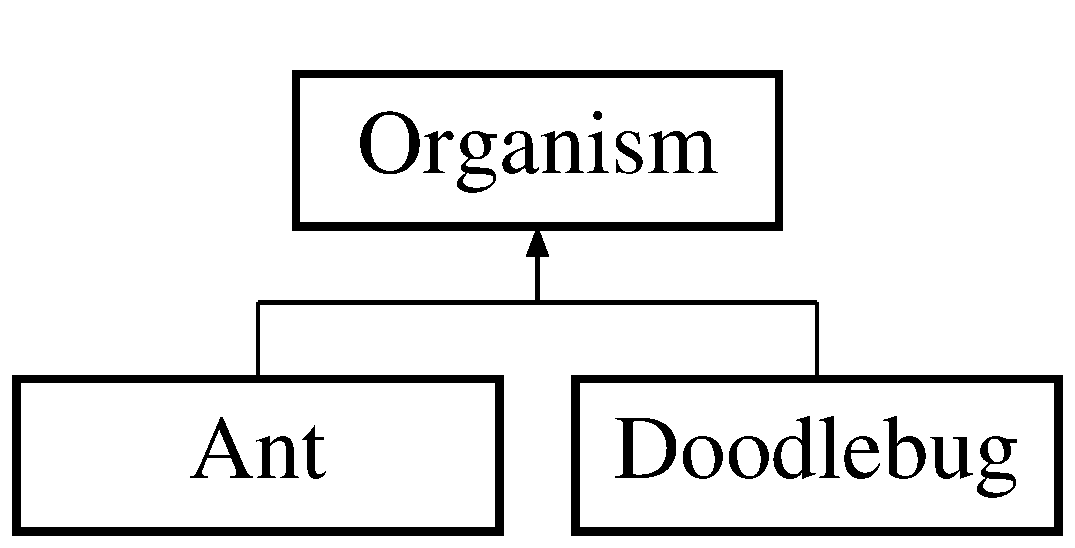
\includegraphics[height=2.000000cm]{classOrganism}
\end{center}
\end{figure}
\subsection*{Public Member Functions}
\begin{DoxyCompactItemize}
\item 
\textbf{ Organism} (int r=0, int c=0, bool s=false)
\item 
int \textbf{ get\+Row} ()
\item 
int \textbf{ get\+Col} ()
\item 
bool \textbf{ get\+Skip} ()
\item 
void \textbf{ set\+Skip} (bool s)
\item 
int \textbf{ get\+Steps\+Since\+Breed} ()
\item 
virtual bool \textbf{ move} (\textbf{ Grid} $\ast$g, int n)=0
\item 
virtual bool \textbf{ breed} (\textbf{ Grid} $\ast$g, int n)=0
\item 
\textbf{ move\+Location} \textbf{ target\+Cell} (\textbf{ Grid} $\ast$g, int r, int c, int n, bool d\+Move)
\item 
virtual \textbf{ $\sim$\+Organism} ()
\end{DoxyCompactItemize}
\subsection*{Protected Attributes}
\begin{DoxyCompactItemize}
\item 
int \textbf{ row}
\item 
int \textbf{ col}
\item 
int \textbf{ steps\+Since\+Breed}
\item 
bool \textbf{ skip}
\item 
int \textbf{ orig\+Row}
\item 
int \textbf{ orig\+Col}
\end{DoxyCompactItemize}


\subsection{Constructor \& Destructor Documentation}
\mbox{\label{classOrganism_ab1b860a67779b82a67a8f41780d2dafe}} 
\index{Organism@{Organism}!Organism@{Organism}}
\index{Organism@{Organism}!Organism@{Organism}}
\subsubsection{Organism()}
{\footnotesize\ttfamily Organism\+::\+Organism (\begin{DoxyParamCaption}\item[{int}]{r = {\ttfamily 0},  }\item[{int}]{c = {\ttfamily 0},  }\item[{bool}]{s = {\ttfamily false} }\end{DoxyParamCaption})}

Constructs an \doxyref{Organism}{p.}{classOrganism}. 
\begin{DoxyParams}{Parameters}
{\em r} & The row of the \doxyref{Organism}{p.}{classOrganism} \\
\hline
{\em c} & The column of the \doxyref{Organism}{p.}{classOrganism} \\
\hline
{\em s} & true if the \doxyref{Organism}{p.}{classOrganism} should be skipped; false otherwise \\
\hline
\end{DoxyParams}


References col, orig\+Col, orig\+Row, row, skip, and steps\+Since\+Breed.

\mbox{\label{classOrganism_aa5aa2e9fc3134358c929fa0c9d230c3b}} 
\index{Organism@{Organism}!````~Organism@{$\sim$\+Organism}}
\index{````~Organism@{$\sim$\+Organism}!Organism@{Organism}}
\subsubsection{$\sim$\+Organism()}
{\footnotesize\ttfamily Organism\+::$\sim$\+Organism (\begin{DoxyParamCaption}{ }\end{DoxyParamCaption})\hspace{0.3cm}{\ttfamily [virtual]}}

Destructs an \doxyref{Organism}{p.}{classOrganism}. 

\subsection{Member Function Documentation}
\mbox{\label{classOrganism_a62e6c3a58974180f039c24889c5e6141}} 
\index{Organism@{Organism}!breed@{breed}}
\index{breed@{breed}!Organism@{Organism}}
\subsubsection{breed()}
{\footnotesize\ttfamily virtual bool Organism\+::breed (\begin{DoxyParamCaption}\item[{\textbf{ Grid} $\ast$}]{g,  }\item[{int}]{n }\end{DoxyParamCaption})\hspace{0.3cm}{\ttfamily [pure virtual]}}



Implemented in \textbf{ Doodlebug} \doxyref{}{p.}{classDoodlebug_a14e41f3251a7a092cec6943a5d7c976d}, and \textbf{ Ant} \doxyref{}{p.}{classAnt_af5d0af0b6e6be8526875773378627666}.

\mbox{\label{classOrganism_a2b8cb6b0955d7997a642cfa27fb93e8e}} 
\index{Organism@{Organism}!get\+Col@{get\+Col}}
\index{get\+Col@{get\+Col}!Organism@{Organism}}
\subsubsection{get\+Col()}
{\footnotesize\ttfamily int Organism\+::get\+Col (\begin{DoxyParamCaption}{ }\end{DoxyParamCaption})}

Gets the column of an \doxyref{Organism}{p.}{classOrganism}. \begin{DoxyReturn}{Returns}
Column of an \doxyref{Organism}{p.}{classOrganism} 
\end{DoxyReturn}


References col.



Referenced by Tests2\+::ants\+Move\+Test(), Tests2\+::get\+Cell\+Occupant\+Ptr\+Test(), Tests2\+::get\+Col\+Test(), Tests2\+::get\+Occupant\+Ptr\+Test(), and Production\+::one\+Doodlebug\+Step().

\mbox{\label{classOrganism_a8189241fd26884ee9c722a081f50387a}} 
\index{Organism@{Organism}!get\+Row@{get\+Row}}
\index{get\+Row@{get\+Row}!Organism@{Organism}}
\subsubsection{get\+Row()}
{\footnotesize\ttfamily int Organism\+::get\+Row (\begin{DoxyParamCaption}{ }\end{DoxyParamCaption})}

Gets the row of an \doxyref{Organism}{p.}{classOrganism}. \begin{DoxyReturn}{Returns}
Row of an \doxyref{Organism}{p.}{classOrganism} 
\end{DoxyReturn}


References row.



Referenced by Tests2\+::ants\+Move\+Test(), Tests2\+::get\+Cell\+Occupant\+Ptr\+Test(), Tests2\+::get\+Occupant\+Ptr\+Test(), Tests2\+::get\+Row\+Test(), and Production\+::one\+Doodlebug\+Step().

\mbox{\label{classOrganism_a99830e9258a1e7fa38ec348636203343}} 
\index{Organism@{Organism}!get\+Skip@{get\+Skip}}
\index{get\+Skip@{get\+Skip}!Organism@{Organism}}
\subsubsection{get\+Skip()}
{\footnotesize\ttfamily bool Organism\+::get\+Skip (\begin{DoxyParamCaption}{ }\end{DoxyParamCaption})}

Gets whether an \doxyref{Organism}{p.}{classOrganism} should be skipped in the loop. \begin{DoxyReturn}{Returns}
true if \doxyref{Organism}{p.}{classOrganism} should be skipped; false otherwise 
\end{DoxyReturn}


References skip.



Referenced by Tests2\+::get\+Skip\+Test(), Production\+::run\+Production(), and Tests2\+::set\+Skip\+Test().

\mbox{\label{classOrganism_a5781744ef51de02648cac785fa658a2a}} 
\index{Organism@{Organism}!get\+Steps\+Since\+Breed@{get\+Steps\+Since\+Breed}}
\index{get\+Steps\+Since\+Breed@{get\+Steps\+Since\+Breed}!Organism@{Organism}}
\subsubsection{get\+Steps\+Since\+Breed()}
{\footnotesize\ttfamily int Organism\+::get\+Steps\+Since\+Breed (\begin{DoxyParamCaption}{ }\end{DoxyParamCaption})}

Gets number of steps since an \doxyref{Organism}{p.}{classOrganism} breed. \begin{DoxyReturn}{Returns}
number of steps since an \doxyref{Organism}{p.}{classOrganism} breed 
\end{DoxyReturn}


References steps\+Since\+Breed.



Referenced by Tests2\+::get\+Steps\+Since\+Breed\+Test(), Production\+::one\+Ant\+Step(), and Production\+::one\+Doodlebug\+Step().

\mbox{\label{classOrganism_a4d767696ff07b88656d35ceb3a0307e6}} 
\index{Organism@{Organism}!move@{move}}
\index{move@{move}!Organism@{Organism}}
\subsubsection{move()}
{\footnotesize\ttfamily virtual bool Organism\+::move (\begin{DoxyParamCaption}\item[{\textbf{ Grid} $\ast$}]{g,  }\item[{int}]{n }\end{DoxyParamCaption})\hspace{0.3cm}{\ttfamily [pure virtual]}}



Implemented in \textbf{ Doodlebug} \doxyref{}{p.}{classDoodlebug_afb9e8b67fd66543f664b855f30546f2e}, and \textbf{ Ant} \doxyref{}{p.}{classAnt_a2f7075f92830a8ce07f868c3feb68720}.

\mbox{\label{classOrganism_adc959f18a4bfe2cda2bbd1e950bd027c}} 
\index{Organism@{Organism}!set\+Skip@{set\+Skip}}
\index{set\+Skip@{set\+Skip}!Organism@{Organism}}
\subsubsection{set\+Skip()}
{\footnotesize\ttfamily void Organism\+::set\+Skip (\begin{DoxyParamCaption}\item[{bool}]{s }\end{DoxyParamCaption})}

Sets whether an \doxyref{Organism}{p.}{classOrganism} should be skipped in the loop. 
\begin{DoxyParams}{Parameters}
{\em s} & true if an \doxyref{Organism}{p.}{classOrganism} should be skipped; false otherwise \\
\hline
\end{DoxyParams}


References skip.



Referenced by Tests2\+::get\+Skip\+Test(), Production\+::run\+Production(), and Tests2\+::set\+Skip\+Test().

\mbox{\label{classOrganism_a551bae612770874f2a0f25897a47dc7c}} 
\index{Organism@{Organism}!target\+Cell@{target\+Cell}}
\index{target\+Cell@{target\+Cell}!Organism@{Organism}}
\subsubsection{target\+Cell()}
{\footnotesize\ttfamily \textbf{ move\+Location} Organism\+::target\+Cell (\begin{DoxyParamCaption}\item[{\textbf{ Grid} $\ast$}]{g,  }\item[{int}]{r,  }\item[{int}]{c,  }\item[{int}]{n,  }\item[{bool}]{d\+Move }\end{DoxyParamCaption})}

Determines the spot that an organism should move to or breed in. Determines if the cell above, below, right, and left are occupied, and out of the empty cells, randomly determines the cell to move to or breed in. If the organism is a \doxyref{Doodlebug}{p.}{classDoodlebug} attempting to move, it will randomly move to an adjacent cell with an \doxyref{Ant}{p.}{classAnt} in it before moving to an empty cell. \doxyref{Organism}{p.}{classOrganism} does not move if all adjacent cells are filled (unless the \doxyref{Organism}{p.}{classOrganism} is a \doxyref{Doodlebug}{p.}{classDoodlebug}, and an \doxyref{Ant}{p.}{classAnt} occupies an adjacent cell). 
\begin{DoxyParams}{Parameters}
{\em g} & The grid with the Organisms \\
\hline
{\em r} & The row of the \doxyref{Organism}{p.}{classOrganism} \\
\hline
{\em c} & The column of the \doxyref{Organism}{p.}{classOrganism} \\
\hline
{\em n} & The number of cells on an edge \\
\hline
{\em d\+Move} & true if the \doxyref{Organism}{p.}{classOrganism} is a \doxyref{Doodlebug}{p.}{classDoodlebug} trying to move; false otherwise \\
\hline
\end{DoxyParams}
\begin{DoxyReturn}{Returns}
stay if \doxyref{Organism}{p.}{classOrganism} cannot move or breed; up if \doxyref{Organism}{p.}{classOrganism} moves or breeds in cell above; right if \doxyref{Organism}{p.}{classOrganism} moves or breeds in cell to the right; down if \doxyref{Organism}{p.}{classOrganism} moves or breeds in cell below; left if \doxyref{Organism}{p.}{classOrganism} moves or breeds in cell to the left 
\end{DoxyReturn}


References ant, down, empty, Grid\+::get\+Cell\+Occupant(), left, right, stay, and up.



Referenced by Ant\+::breed(), Doodlebug\+::breed(), Ant\+::move(), Doodlebug\+::move(), and Tests2\+::target\+Cell\+Test().



\subsection{Field Documentation}
\mbox{\label{classOrganism_a8f36f6e8f707ab4bc34e5edd31bfec07}} 
\index{Organism@{Organism}!col@{col}}
\index{col@{col}!Organism@{Organism}}
\subsubsection{col}
{\footnotesize\ttfamily int Organism\+::col\hspace{0.3cm}{\ttfamily [protected]}}



Referenced by Ant\+::breed(), Doodlebug\+::breed(), Doodlebug\+::eat(), get\+Col(), Ant\+::move(), Doodlebug\+::move(), and Organism().

\mbox{\label{classOrganism_aea6f01ae34268ee8a15997688b38f8f5}} 
\index{Organism@{Organism}!orig\+Col@{orig\+Col}}
\index{orig\+Col@{orig\+Col}!Organism@{Organism}}
\subsubsection{orig\+Col}
{\footnotesize\ttfamily int Organism\+::orig\+Col\hspace{0.3cm}{\ttfamily [protected]}}



Referenced by Ant\+::breed(), Doodlebug\+::breed(), Ant\+::move(), Doodlebug\+::move(), and Organism().

\mbox{\label{classOrganism_ae58dffec529b268348c378b6be5e39ec}} 
\index{Organism@{Organism}!orig\+Row@{orig\+Row}}
\index{orig\+Row@{orig\+Row}!Organism@{Organism}}
\subsubsection{orig\+Row}
{\footnotesize\ttfamily int Organism\+::orig\+Row\hspace{0.3cm}{\ttfamily [protected]}}



Referenced by Ant\+::breed(), Doodlebug\+::breed(), Ant\+::move(), Doodlebug\+::move(), and Organism().

\mbox{\label{classOrganism_aa298debd9753da69e00e575f5ab2a73f}} 
\index{Organism@{Organism}!row@{row}}
\index{row@{row}!Organism@{Organism}}
\subsubsection{row}
{\footnotesize\ttfamily int Organism\+::row\hspace{0.3cm}{\ttfamily [protected]}}



Referenced by Ant\+::breed(), Doodlebug\+::breed(), Doodlebug\+::eat(), get\+Row(), Ant\+::move(), Doodlebug\+::move(), and Organism().

\mbox{\label{classOrganism_a8b982b34f4923ab00a5c7d0013ceaf9e}} 
\index{Organism@{Organism}!skip@{skip}}
\index{skip@{skip}!Organism@{Organism}}
\subsubsection{skip}
{\footnotesize\ttfamily bool Organism\+::skip\hspace{0.3cm}{\ttfamily [protected]}}



Referenced by get\+Skip(), Ant\+::move(), Doodlebug\+::move(), Organism(), and set\+Skip().

\mbox{\label{classOrganism_aed086b9d4cb09047f37dc9120aeb10e6}} 
\index{Organism@{Organism}!steps\+Since\+Breed@{steps\+Since\+Breed}}
\index{steps\+Since\+Breed@{steps\+Since\+Breed}!Organism@{Organism}}
\subsubsection{steps\+Since\+Breed}
{\footnotesize\ttfamily int Organism\+::steps\+Since\+Breed\hspace{0.3cm}{\ttfamily [protected]}}



Referenced by Ant\+::breed(), Doodlebug\+::breed(), get\+Steps\+Since\+Breed(), Ant\+::move(), Doodlebug\+::move(), and Organism().



The documentation for this class was generated from the following files\+:\begin{DoxyCompactItemize}
\item 
\textbf{ Organism.\+h}\item 
\textbf{ Organism.\+cpp}\end{DoxyCompactItemize}

\section{Production Class Reference}
\label{classProduction}\index{Production@{Production}}


{\ttfamily \#include $<$Production.\+h$>$}

\subsection*{Public Member Functions}
\begin{DoxyCompactItemize}
\item 
\textbf{ Production} (int argc, char $\ast$argv[$\,$])
\item 
bool \textbf{ run\+Production} ()
\item 
bool \textbf{ one\+Doodlebug\+Step} (\textbf{ Grid} $\ast$g, int r, int c)
\item 
bool \textbf{ one\+Ant\+Step} (\textbf{ Grid} $\ast$g, int r, int c)
\item 
virtual \textbf{ $\sim$\+Production} ()
\end{DoxyCompactItemize}
\subsection*{Private Attributes}
\begin{DoxyCompactItemize}
\item 
int \textbf{ grid\+Size}
\item 
int \textbf{ num\+Doodlebugs}
\item 
int \textbf{ num\+Ants}
\item 
int \textbf{ num\+Time\+Steps}
\item 
int \textbf{ seed}
\item 
int \textbf{ pause}
\end{DoxyCompactItemize}


\subsection{Constructor \& Destructor Documentation}
\mbox{\label{classProduction_a24439558b7672feaea80dc0ab1b53ff2}} 
\index{Production@{Production}!Production@{Production}}
\index{Production@{Production}!Production@{Production}}
\subsubsection{Production()}
{\footnotesize\ttfamily Production\+::\+Production (\begin{DoxyParamCaption}\item[{int}]{argc,  }\item[{char $\ast$}]{argv[$\,$] }\end{DoxyParamCaption})}

Constructs a \doxyref{Production}{p.}{classProduction} 
\begin{DoxyParams}{Parameters}
{\em argc} & Number of arguments on the Command Line \\
\hline
{\em argv} & Array of arguments on the Command Line \\
\hline
\end{DoxyParams}


References grid\+Size, num\+Ants, num\+Doodlebugs, num\+Time\+Steps, pause, and seed.



Referenced by main().

\mbox{\label{classProduction_ab5b3060f9e0a2bc189844e426d693dab}} 
\index{Production@{Production}!````~Production@{$\sim$\+Production}}
\index{````~Production@{$\sim$\+Production}!Production@{Production}}
\subsubsection{$\sim$\+Production()}
{\footnotesize\ttfamily Production\+::$\sim$\+Production (\begin{DoxyParamCaption}{ }\end{DoxyParamCaption})\hspace{0.3cm}{\ttfamily [virtual]}}

Destructs \doxyref{Production}{p.}{classProduction}. 

Referenced by Tests2\+::get\+Steps\+Since\+Ate\+Test(), Tests2\+::get\+Steps\+Since\+Breed\+Test(), main(), Tests2\+::one\+Ant\+Step\+Test(), Tests2\+::one\+Doodlebug\+Step\+Test(), and Tests2\+::run\+Production\+Test().



\subsection{Member Function Documentation}
\mbox{\label{classProduction_ab7c0ed9fcb1e452334b491cb8afcd6bc}} 
\index{Production@{Production}!one\+Ant\+Step@{one\+Ant\+Step}}
\index{one\+Ant\+Step@{one\+Ant\+Step}!Production@{Production}}
\subsubsection{one\+Ant\+Step()}
{\footnotesize\ttfamily bool Production\+::one\+Ant\+Step (\begin{DoxyParamCaption}\item[{\textbf{ Grid} $\ast$}]{g,  }\item[{int}]{r,  }\item[{int}]{c }\end{DoxyParamCaption})}

Simulates an \doxyref{Ant}{p.}{classAnt} for one step. 
\begin{DoxyParams}{Parameters}
{\em g} & \doxyref{Grid}{p.}{classGrid} that contains the organisms \\
\hline
{\em r} & Row of the \doxyref{Ant}{p.}{classAnt} \\
\hline
{\em c} & Column of the \doxyref{Ant}{p.}{classAnt} \\
\hline
\end{DoxyParams}
\begin{DoxyReturn}{Returns}
true if birth was given; false otherwise; 
\end{DoxyReturn}


References Ant\+::breed(), Grid\+::get\+Cell\+Occupant\+Ptr(), Organism\+::get\+Steps\+Since\+Breed(), grid\+Size, and Ant\+::move().



Referenced by Tests2\+::get\+Steps\+Since\+Breed\+Test(), Tests2\+::one\+Ant\+Step\+Test(), and run\+Production().

\mbox{\label{classProduction_aed65add8e44260bf21000091cf68ef93}} 
\index{Production@{Production}!one\+Doodlebug\+Step@{one\+Doodlebug\+Step}}
\index{one\+Doodlebug\+Step@{one\+Doodlebug\+Step}!Production@{Production}}
\subsubsection{one\+Doodlebug\+Step()}
{\footnotesize\ttfamily bool Production\+::one\+Doodlebug\+Step (\begin{DoxyParamCaption}\item[{\textbf{ Grid} $\ast$}]{g,  }\item[{int}]{r,  }\item[{int}]{c }\end{DoxyParamCaption})}

Simulates a \doxyref{Doodlebug}{p.}{classDoodlebug} for one step. 
\begin{DoxyParams}{Parameters}
{\em g} & \doxyref{Grid}{p.}{classGrid} that contains the organisms \\
\hline
{\em r} & Row of the \doxyref{Doodlebug}{p.}{classDoodlebug} \\
\hline
{\em c} & Column of the \doxyref{Doodlebug}{p.}{classDoodlebug} \\
\hline
\end{DoxyParams}
\begin{DoxyReturn}{Returns}
true if birth was given; false otherwise; 
\end{DoxyReturn}


References Doodlebug\+::breed(), empty, Grid\+::get\+Cell\+Occupant\+Ptr(), Organism\+::get\+Col(), Organism\+::get\+Row(), Doodlebug\+::get\+Steps\+Since\+Ate(), Organism\+::get\+Steps\+Since\+Breed(), grid\+Size, Doodlebug\+::move(), and Grid\+::set\+Cell\+Occupant().



Referenced by Tests2\+::doodle\+Eat\+Test(), Tests2\+::get\+Steps\+Since\+Ate\+Test(), Tests2\+::one\+Doodlebug\+Step\+Test(), and run\+Production().

\mbox{\label{classProduction_a1d66853eafae2580089eff44f12f07ba}} 
\index{Production@{Production}!run\+Production@{run\+Production}}
\index{run\+Production@{run\+Production}!Production@{Production}}
\subsubsection{run\+Production()}
{\footnotesize\ttfamily bool Production\+::run\+Production (\begin{DoxyParamCaption}{ }\end{DoxyParamCaption})}

Main \doxyref{Production}{p.}{classProduction} method. \begin{DoxyReturn}{Returns}
true if production seemed to work; false otherwise 
\end{DoxyReturn}
We iterate through all of the Cells of the \doxyref{Grid}{p.}{classGrid} and perform all of 

References ant, doodlebug, Grid\+::get\+Cell\+Occupant(), Grid\+::get\+Cell\+Occupant\+Ptr(), Organism\+::get\+Skip(), grid\+Size, Grid\+::init\+Grid(), num\+Ants, num\+Doodlebugs, num\+Time\+Steps, one\+Ant\+Step(), one\+Doodlebug\+Step(), pause, Grid\+::print\+Grid(), seed, and Organism\+::set\+Skip().



Referenced by main(), and Tests2\+::run\+Production\+Test().



\subsection{Field Documentation}
\mbox{\label{classProduction_aec26b656d2e7519d1a1898810bd1c0da}} 
\index{Production@{Production}!grid\+Size@{grid\+Size}}
\index{grid\+Size@{grid\+Size}!Production@{Production}}
\subsubsection{grid\+Size}
{\footnotesize\ttfamily int Production\+::grid\+Size\hspace{0.3cm}{\ttfamily [private]}}



Referenced by one\+Ant\+Step(), one\+Doodlebug\+Step(), Production(), and run\+Production().

\mbox{\label{classProduction_a9bf1f5e66a3a787f08d37d5ef06cf8b6}} 
\index{Production@{Production}!num\+Ants@{num\+Ants}}
\index{num\+Ants@{num\+Ants}!Production@{Production}}
\subsubsection{num\+Ants}
{\footnotesize\ttfamily int Production\+::num\+Ants\hspace{0.3cm}{\ttfamily [private]}}



Referenced by Production(), and run\+Production().

\mbox{\label{classProduction_a3bfd9e01f9f73efd1f92176e5f7458eb}} 
\index{Production@{Production}!num\+Doodlebugs@{num\+Doodlebugs}}
\index{num\+Doodlebugs@{num\+Doodlebugs}!Production@{Production}}
\subsubsection{num\+Doodlebugs}
{\footnotesize\ttfamily int Production\+::num\+Doodlebugs\hspace{0.3cm}{\ttfamily [private]}}



Referenced by Production(), and run\+Production().

\mbox{\label{classProduction_a079f2c4ddd0af799fd4c11b7a96a3065}} 
\index{Production@{Production}!num\+Time\+Steps@{num\+Time\+Steps}}
\index{num\+Time\+Steps@{num\+Time\+Steps}!Production@{Production}}
\subsubsection{num\+Time\+Steps}
{\footnotesize\ttfamily int Production\+::num\+Time\+Steps\hspace{0.3cm}{\ttfamily [private]}}



Referenced by Production(), and run\+Production().

\mbox{\label{classProduction_af570feb7415a4d5b1a9176dacd9d6b64}} 
\index{Production@{Production}!pause@{pause}}
\index{pause@{pause}!Production@{Production}}
\subsubsection{pause}
{\footnotesize\ttfamily int Production\+::pause\hspace{0.3cm}{\ttfamily [private]}}



Referenced by Production(), and run\+Production().

\mbox{\label{classProduction_adb474287b0143fccb9d440ccc54ba624}} 
\index{Production@{Production}!seed@{seed}}
\index{seed@{seed}!Production@{Production}}
\subsubsection{seed}
{\footnotesize\ttfamily int Production\+::seed\hspace{0.3cm}{\ttfamily [private]}}



Referenced by Production(), and run\+Production().



The documentation for this class was generated from the following files\+:\begin{DoxyCompactItemize}
\item 
\textbf{ Production.\+h}\item 
\textbf{ Production.\+cpp}\end{DoxyCompactItemize}

\section{Tests2 Class Reference}
\label{classTests2}\index{Tests2@{Tests2}}


{\ttfamily \#include $<$Tests2.\+h$>$}

\subsection*{Public Member Functions}
\begin{DoxyCompactItemize}
\item 
\textbf{ Tests2} ()
\item 
bool \textbf{ do\+Tests} ()
\item 
bool \textbf{ run\+Production\+Test} ()
\item 
bool \textbf{ one\+Doodlebug\+Step\+Test} ()
\item 
bool \textbf{ one\+Ant\+Step\+Test} ()
\item 
bool \textbf{ grid\+Test} ()
\item 
bool \textbf{ get\+Cell\+Occupant\+Test} ()
\item 
bool \textbf{ set\+Cell\+Occupant\+Test} ()
\item 
bool \textbf{ get\+Cell\+Occupant\+Ptr\+Test} ()
\item 
bool \textbf{ init\+Grid\+Test} ()
\item 
bool \textbf{ print\+Grid} ()
\item 
bool \textbf{ get\+Occupant\+Test} ()
\item 
bool \textbf{ set\+Occupant\+Test} ()
\item 
bool \textbf{ get\+Occupant\+Ptr\+Test} ()
\item 
bool \textbf{ get\+Row\+Test} ()
\item 
bool \textbf{ get\+Col\+Test} ()
\item 
bool \textbf{ get\+Skip\+Test} ()
\item 
bool \textbf{ set\+Skip\+Test} ()
\item 
bool \textbf{ get\+Steps\+Since\+Breed\+Test} ()
\item 
bool \textbf{ target\+Cell\+Test} ()
\item 
bool \textbf{ make\+Ants\+Test} ()
\item 
bool \textbf{ ants\+Move\+Test} ()
\item 
bool \textbf{ ants\+Breed\+Test} ()
\item 
bool \textbf{ make\+Doodles\+Test} ()
\item 
bool \textbf{ doodle\+Move\+Test} ()
\item 
bool \textbf{ doodle\+Breed\+Test} ()
\item 
bool \textbf{ doodle\+Eat\+Test} ()
\item 
bool \textbf{ get\+Steps\+Since\+Ate\+Test} ()
\item 
virtual \textbf{ $\sim$\+Tests2} ()
\end{DoxyCompactItemize}


\subsection{Constructor \& Destructor Documentation}
\mbox{\label{classTests2_a6d7d8d248dd3d544199769baa1face60}} 
\index{Tests2@{Tests2}!Tests2@{Tests2}}
\index{Tests2@{Tests2}!Tests2@{Tests2}}
\subsubsection{Tests2()}
{\footnotesize\ttfamily Tests2\+::\+Tests2 (\begin{DoxyParamCaption}{ }\end{DoxyParamCaption})}

Constructs a Test. \mbox{\label{classTests2_abed1a850ef511b7c06ae418cb3bbd5d9}} 
\index{Tests2@{Tests2}!````~Tests2@{$\sim$\+Tests2}}
\index{````~Tests2@{$\sim$\+Tests2}!Tests2@{Tests2}}
\subsubsection{$\sim$\+Tests2()}
{\footnotesize\ttfamily Tests2\+::$\sim$\+Tests2 (\begin{DoxyParamCaption}{ }\end{DoxyParamCaption})\hspace{0.3cm}{\ttfamily [virtual]}}

Destructs a Test. 

Referenced by main().



\subsection{Member Function Documentation}
\mbox{\label{classTests2_a21e7692afbdfb694caf370670cbeb7d4}} 
\index{Tests2@{Tests2}!ants\+Breed\+Test@{ants\+Breed\+Test}}
\index{ants\+Breed\+Test@{ants\+Breed\+Test}!Tests2@{Tests2}}
\subsubsection{ants\+Breed\+Test()}
{\footnotesize\ttfamily bool Tests2\+::ants\+Breed\+Test (\begin{DoxyParamCaption}{ }\end{DoxyParamCaption})}

Tests that an \doxyref{Ant}{p.}{classAnt} can breed and produce a new \doxyref{Ant}{p.}{classAnt} in an adjacent \doxyref{Cell}{p.}{classCell} \begin{DoxyReturn}{Returns}
true if the test passes; false otherwise
\end{DoxyReturn}
Initial \doxyref{Grid}{p.}{classGrid}\+: 0123456789 0 -\/-\/-\/-\/-\/-\/-\/--- 0 1 -\/\+A\+A-\/\+A-\/-\/--- 1 A = \doxyref{Ant}{p.}{classAnt} 2 --A-\/-\/-\/-\/--- 2 D = \doxyref{Doodlebug}{p.}{classDoodlebug} 3 -\/-\/-\/-\/-\/-\/-\/--- 3 -\/ = empty 4 -\/-\/-\/-\/---A\+D-\/ 4 5 -\/-\/-\/---A\+A\+A-\/ 5 6 -\/-\/-\/-\/---A-- 6 7 -\/---A-\/-\/--- 7 8 -\/-\/-\/-\/-\/-\/-\/--- 8 9 -\/-\/-\/-\/-\/-\/---A 9 0123456789 

References ant, Ant\+::breed(), doodlebug, Grid\+::get\+Cell\+Occupant(), and Grid\+::set\+Cell\+Occupant().



Referenced by do\+Tests().

\mbox{\label{classTests2_a7694d2797eba6fadc40234d527f6afbe}} 
\index{Tests2@{Tests2}!ants\+Move\+Test@{ants\+Move\+Test}}
\index{ants\+Move\+Test@{ants\+Move\+Test}!Tests2@{Tests2}}
\subsubsection{ants\+Move\+Test()}
{\footnotesize\ttfamily bool Tests2\+::ants\+Move\+Test (\begin{DoxyParamCaption}{ }\end{DoxyParamCaption})}

Tests that an \doxyref{Ant}{p.}{classAnt} can move to an adjacent spot \begin{DoxyReturn}{Returns}
true if the test passes; false otherwise
\end{DoxyReturn}
Initial \doxyref{Grid}{p.}{classGrid}\+: 0123456789 0 -\/-\/-\/-\/-\/-\/-\/--- 0 1 -\/\+A\+A-\/\+D-\/-\/--- 1 A = \doxyref{Ant}{p.}{classAnt} 2 --A-\/-\/-\/-\/--- 2 D = \doxyref{Doodlebug}{p.}{classDoodlebug} 3 -\/-\/-\/-\/-\/-\/-\/--- 3 -\/ = empty 4 -\/-\/-\/-\/---A-- 4 5 -\/-\/-\/---A\+A\+A-\/ 5 6 -\/-\/-\/-\/---A-- 6 7 -\/---A-\/-\/--- 7 8 -\/-\/-\/-\/-\/-\/-\/--- 8 9 -\/-\/-\/-\/-\/-\/---A 9 0123456789 

References ant, doodlebug, Organism\+::get\+Col(), Organism\+::get\+Row(), Ant\+::move(), and Grid\+::set\+Cell\+Occupant().



Referenced by do\+Tests().

\mbox{\label{classTests2_a317dc926bf93038f188c999df7a85682}} 
\index{Tests2@{Tests2}!doodle\+Breed\+Test@{doodle\+Breed\+Test}}
\index{doodle\+Breed\+Test@{doodle\+Breed\+Test}!Tests2@{Tests2}}
\subsubsection{doodle\+Breed\+Test()}
{\footnotesize\ttfamily bool Tests2\+::doodle\+Breed\+Test (\begin{DoxyParamCaption}{ }\end{DoxyParamCaption})}

Tests that a \doxyref{Doodlebug}{p.}{classDoodlebug} gives birth to a new \doxyref{Doodlebug}{p.}{classDoodlebug} in an adjacent \doxyref{Cell}{p.}{classCell} \begin{DoxyReturn}{Returns}
true if the test passes; false otherwise
\end{DoxyReturn}
Initial \doxyref{Grid}{p.}{classGrid}\+: 0123456789 0 -\/-\/-\/-\/-\/-\/-\/--- 0 1 -\/\+A\+A-\/\+D-\/-\/--- 1 A = \doxyref{Ant}{p.}{classAnt} 2 --A-\/-\/-\/-\/--- 2 D = \doxyref{Doodlebug}{p.}{classDoodlebug} 3 -\/-\/-\/-\/-\/-\/-\/--- 3 -\/ = empty 4 -\/-\/-\/-\/---A\+D-\/ 4 5 -\/-\/-\/---A\+D\+D-\/ 5 6 -\/-\/-\/-\/---A-- 6 7 -\/---A-\/-\/--- 7 8 -\/-\/-\/-\/-\/-\/-\/--- 8 9 -\/-\/-\/-\/-\/-\/---D 9 0123456789 

References ant, Doodlebug\+::breed(), doodlebug, Grid\+::get\+Cell\+Occupant(), and Grid\+::set\+Cell\+Occupant().



Referenced by do\+Tests().

\mbox{\label{classTests2_ae35f30e7d95e581cc4ce1316409c71ac}} 
\index{Tests2@{Tests2}!doodle\+Eat\+Test@{doodle\+Eat\+Test}}
\index{doodle\+Eat\+Test@{doodle\+Eat\+Test}!Tests2@{Tests2}}
\subsubsection{doodle\+Eat\+Test()}
{\footnotesize\ttfamily bool Tests2\+::doodle\+Eat\+Test (\begin{DoxyParamCaption}{ }\end{DoxyParamCaption})}

Tests that a \doxyref{Doodlebug}{p.}{classDoodlebug} properly eats \begin{DoxyReturn}{Returns}
true if the test passes; false otherwise 
\end{DoxyReturn}


References ant, doodlebug, Grid\+::get\+Cell\+Occupant(), Production\+::one\+Doodlebug\+Step(), Grid\+::set\+Cell\+Occupant(), and Grid\+::$\sim$\+Grid().



Referenced by do\+Tests().

\mbox{\label{classTests2_a2143f2192836626e7214d37b504df381}} 
\index{Tests2@{Tests2}!doodle\+Move\+Test@{doodle\+Move\+Test}}
\index{doodle\+Move\+Test@{doodle\+Move\+Test}!Tests2@{Tests2}}
\subsubsection{doodle\+Move\+Test()}
{\footnotesize\ttfamily bool Tests2\+::doodle\+Move\+Test (\begin{DoxyParamCaption}{ }\end{DoxyParamCaption})}

Tests that a \doxyref{Doodlebug}{p.}{classDoodlebug} can correctly move to an adjacent Dell \begin{DoxyReturn}{Returns}
true if the test passes; false otherwise
\end{DoxyReturn}
Initial \doxyref{Grid}{p.}{classGrid}\+: 0123456789 0 -\/-\/-\/-\/-\/-\/-\/--- 0 1 -\/\+A\+A-\/\+D-\/-\/--- 1 A = \doxyref{Ant}{p.}{classAnt} 2 --A-\/-\/-\/-\/--- 2 D = \doxyref{Doodlebug}{p.}{classDoodlebug} 3 -\/-\/-\/-\/-\/-\/-\/--- 3 -\/ = empty 4 -\/-\/-\/-\/---A\+D-\/ 4 5 -\/-\/-\/---A\+D\+D-\/ 5 6 -\/-\/-\/-\/---A-- 6 7 -\/---A-\/-\/--- 7 8 -\/-\/-\/-\/-\/-\/-\/--- 8 9 -\/-\/-\/-\/-\/-\/---D 9 0123456789 

References ant, doodlebug, Grid\+::get\+Cell\+Occupant(), Doodlebug\+::move(), and Grid\+::set\+Cell\+Occupant().



Referenced by do\+Tests().

\mbox{\label{classTests2_a7392382310966597d685c8aa3a4a2f88}} 
\index{Tests2@{Tests2}!do\+Tests@{do\+Tests}}
\index{do\+Tests@{do\+Tests}!Tests2@{Tests2}}
\subsubsection{do\+Tests()}
{\footnotesize\ttfamily bool Tests2\+::do\+Tests (\begin{DoxyParamCaption}{ }\end{DoxyParamCaption})}

Performs the tests. \begin{DoxyReturn}{Returns}
true if all tests passes; false otherwise 
\end{DoxyReturn}


References ants\+Breed\+Test(), ants\+Move\+Test(), doodle\+Breed\+Test(), doodle\+Eat\+Test(), doodle\+Move\+Test(), get\+Cell\+Occupant\+Ptr\+Test(), get\+Cell\+Occupant\+Test(), get\+Col\+Test(), get\+Occupant\+Ptr\+Test(), get\+Occupant\+Test(), get\+Row\+Test(), get\+Skip\+Test(), get\+Steps\+Since\+Ate\+Test(), get\+Steps\+Since\+Breed\+Test(), grid\+Test(), init\+Grid\+Test(), make\+Ants\+Test(), make\+Doodles\+Test(), one\+Ant\+Step\+Test(), one\+Doodlebug\+Step\+Test(), print\+Grid(), run\+Production\+Test(), set\+Cell\+Occupant\+Test(), set\+Occupant\+Test(), set\+Skip\+Test(), and target\+Cell\+Test().



Referenced by main().

\mbox{\label{classTests2_a2212e5e8179c34d08d392d72f7861046}} 
\index{Tests2@{Tests2}!get\+Cell\+Occupant\+Ptr\+Test@{get\+Cell\+Occupant\+Ptr\+Test}}
\index{get\+Cell\+Occupant\+Ptr\+Test@{get\+Cell\+Occupant\+Ptr\+Test}!Tests2@{Tests2}}
\subsubsection{get\+Cell\+Occupant\+Ptr\+Test()}
{\footnotesize\ttfamily bool Tests2\+::get\+Cell\+Occupant\+Ptr\+Test (\begin{DoxyParamCaption}{ }\end{DoxyParamCaption})}

Tests that the function correctly gets the pointer to a \doxyref{Cell}{p.}{classCell}. \begin{DoxyReturn}{Returns}
true if tests passes; false otherwise 
\end{DoxyReturn}


References ant, doodlebug, Grid\+::get\+Cell\+Occupant\+Ptr(), Organism\+::get\+Col(), Organism\+::get\+Row(), Grid\+::set\+Cell\+Occupant(), and Grid\+::$\sim$\+Grid().



Referenced by do\+Tests().

\mbox{\label{classTests2_af7092468fb374e2687f13170998e25be}} 
\index{Tests2@{Tests2}!get\+Cell\+Occupant\+Test@{get\+Cell\+Occupant\+Test}}
\index{get\+Cell\+Occupant\+Test@{get\+Cell\+Occupant\+Test}!Tests2@{Tests2}}
\subsubsection{get\+Cell\+Occupant\+Test()}
{\footnotesize\ttfamily bool Tests2\+::get\+Cell\+Occupant\+Test (\begin{DoxyParamCaption}{ }\end{DoxyParamCaption})}

Tests that the function correctly gets the cell occupant type. \begin{DoxyReturn}{Returns}
true if tests passes; false otherwise 
\end{DoxyReturn}


References ant, doodlebug, empty, Grid\+::get\+Cell\+Occupant(), Grid\+::set\+Cell\+Occupant(), and Grid\+::$\sim$\+Grid().



Referenced by do\+Tests().

\mbox{\label{classTests2_a4e8f3fec549826ab1f3e68c157fe07a8}} 
\index{Tests2@{Tests2}!get\+Col\+Test@{get\+Col\+Test}}
\index{get\+Col\+Test@{get\+Col\+Test}!Tests2@{Tests2}}
\subsubsection{get\+Col\+Test()}
{\footnotesize\ttfamily bool Tests2\+::get\+Col\+Test (\begin{DoxyParamCaption}{ }\end{DoxyParamCaption})}

Tests that the function returns the correct column number that an \doxyref{Organism}{p.}{classOrganism} is occupying. \begin{DoxyReturn}{Returns}
true if tests passes; false otherwise 
\end{DoxyReturn}


References Organism\+::get\+Col().



Referenced by do\+Tests().

\mbox{\label{classTests2_ad8b6805a66d039a0abbfd23828d5f650}} 
\index{Tests2@{Tests2}!get\+Occupant\+Ptr\+Test@{get\+Occupant\+Ptr\+Test}}
\index{get\+Occupant\+Ptr\+Test@{get\+Occupant\+Ptr\+Test}!Tests2@{Tests2}}
\subsubsection{get\+Occupant\+Ptr\+Test()}
{\footnotesize\ttfamily bool Tests2\+::get\+Occupant\+Ptr\+Test (\begin{DoxyParamCaption}{ }\end{DoxyParamCaption})}

Tests that the function returns the correct pointer to an \doxyref{Organism}{p.}{classOrganism}. \begin{DoxyReturn}{Returns}
true if tests passes; false otherwise 
\end{DoxyReturn}


References ant, doodlebug, Organism\+::get\+Col(), Cell\+::get\+Occupant\+Ptr(), Organism\+::get\+Row(), Cell\+::set\+Occupant(), and Cell\+::$\sim$\+Cell().



Referenced by do\+Tests().

\mbox{\label{classTests2_a04dc1a9e75200929fb5365606f981a47}} 
\index{Tests2@{Tests2}!get\+Occupant\+Test@{get\+Occupant\+Test}}
\index{get\+Occupant\+Test@{get\+Occupant\+Test}!Tests2@{Tests2}}
\subsubsection{get\+Occupant\+Test()}
{\footnotesize\ttfamily bool Tests2\+::get\+Occupant\+Test (\begin{DoxyParamCaption}{ }\end{DoxyParamCaption})}

Tests that the function correctly gets the \doxyref{Organism}{p.}{classOrganism} type of a c\+Cll. \begin{DoxyReturn}{Returns}
true if tests passes; false otherwise 
\end{DoxyReturn}


References ant, doodlebug, empty, Cell\+::get\+Occupant(), and Cell\+::set\+Occupant().



Referenced by do\+Tests().

\mbox{\label{classTests2_a73020e99dc356b1e5e94c43d09748af3}} 
\index{Tests2@{Tests2}!get\+Row\+Test@{get\+Row\+Test}}
\index{get\+Row\+Test@{get\+Row\+Test}!Tests2@{Tests2}}
\subsubsection{get\+Row\+Test()}
{\footnotesize\ttfamily bool Tests2\+::get\+Row\+Test (\begin{DoxyParamCaption}{ }\end{DoxyParamCaption})}

Tests that the function returns the correct row number that the \doxyref{Organism}{p.}{classOrganism} is occupying. \begin{DoxyReturn}{Returns}
true if tests passes; false otherwise 
\end{DoxyReturn}


References Organism\+::get\+Row().



Referenced by do\+Tests().

\mbox{\label{classTests2_a445d300432cc58396e8090e96b2f8230}} 
\index{Tests2@{Tests2}!get\+Skip\+Test@{get\+Skip\+Test}}
\index{get\+Skip\+Test@{get\+Skip\+Test}!Tests2@{Tests2}}
\subsubsection{get\+Skip\+Test()}
{\footnotesize\ttfamily bool Tests2\+::get\+Skip\+Test (\begin{DoxyParamCaption}{ }\end{DoxyParamCaption})}

Tests that the skip variable returns the correct value. \begin{DoxyReturn}{Returns}
true if tests passes; false otherwise 
\end{DoxyReturn}


References Organism\+::get\+Skip(), and Organism\+::set\+Skip().



Referenced by do\+Tests().

\mbox{\label{classTests2_abdbf5e30603584234924f4c8800e94fe}} 
\index{Tests2@{Tests2}!get\+Steps\+Since\+Ate\+Test@{get\+Steps\+Since\+Ate\+Test}}
\index{get\+Steps\+Since\+Ate\+Test@{get\+Steps\+Since\+Ate\+Test}!Tests2@{Tests2}}
\subsubsection{get\+Steps\+Since\+Ate\+Test()}
{\footnotesize\ttfamily bool Tests2\+::get\+Steps\+Since\+Ate\+Test (\begin{DoxyParamCaption}{ }\end{DoxyParamCaption})}

Tests that the number of steps since a \doxyref{Doodlebug}{p.}{classDoodlebug} ate is correct \begin{DoxyReturn}{Returns}
true if tests passes; false otherwise 
\end{DoxyReturn}


References doodlebug, Doodlebug\+::get\+Steps\+Since\+Ate(), Production\+::one\+Doodlebug\+Step(), Grid\+::set\+Cell\+Occupant(), Grid\+::$\sim$\+Grid(), and Production\+::$\sim$\+Production().



Referenced by do\+Tests().

\mbox{\label{classTests2_a677e77e398237e09838dfe9998c4af0a}} 
\index{Tests2@{Tests2}!get\+Steps\+Since\+Breed\+Test@{get\+Steps\+Since\+Breed\+Test}}
\index{get\+Steps\+Since\+Breed\+Test@{get\+Steps\+Since\+Breed\+Test}!Tests2@{Tests2}}
\subsubsection{get\+Steps\+Since\+Breed\+Test()}
{\footnotesize\ttfamily bool Tests2\+::get\+Steps\+Since\+Breed\+Test (\begin{DoxyParamCaption}{ }\end{DoxyParamCaption})}

Tests that the number of steps since an \doxyref{Organism}{p.}{classOrganism} breed is correct. \begin{DoxyReturn}{Returns}
true if tests passes; false otherwise 
\end{DoxyReturn}


References ant, Organism\+::get\+Steps\+Since\+Breed(), Production\+::one\+Ant\+Step(), Grid\+::set\+Cell\+Occupant(), Grid\+::$\sim$\+Grid(), and Production\+::$\sim$\+Production().



Referenced by do\+Tests().

\mbox{\label{classTests2_afe90de3a79c4105e63205cb8f019bbb2}} 
\index{Tests2@{Tests2}!grid\+Test@{grid\+Test}}
\index{grid\+Test@{grid\+Test}!Tests2@{Tests2}}
\subsubsection{grid\+Test()}
{\footnotesize\ttfamily bool Tests2\+::grid\+Test (\begin{DoxyParamCaption}{ }\end{DoxyParamCaption})}

Tests grid initialization and adding organisms. \begin{DoxyReturn}{Returns}
true if test passes; false otherwise 
\end{DoxyReturn}


References ant, doodlebug, empty, Grid\+::get\+Cell\+Occupant(), Grid\+::set\+Cell\+Occupant(), and Grid\+::$\sim$\+Grid().



Referenced by do\+Tests().

\mbox{\label{classTests2_a01c2990964cc59c5c1366b3f296703a3}} 
\index{Tests2@{Tests2}!init\+Grid\+Test@{init\+Grid\+Test}}
\index{init\+Grid\+Test@{init\+Grid\+Test}!Tests2@{Tests2}}
\subsubsection{init\+Grid\+Test()}
{\footnotesize\ttfamily bool Tests2\+::init\+Grid\+Test (\begin{DoxyParamCaption}{ }\end{DoxyParamCaption})}

Tests that the \doxyref{Grid}{p.}{classGrid} is correctly initialized. \begin{DoxyReturn}{Returns}
true if tests passes; false otherwise 
\end{DoxyReturn}


References empty, Grid\+::get\+Cell\+Occupant(), Grid\+::get\+Cell\+Occupant\+Ptr(), and Grid\+::$\sim$\+Grid().



Referenced by do\+Tests().

\mbox{\label{classTests2_aa4d40396194cf770aa82dc11b449ea62}} 
\index{Tests2@{Tests2}!make\+Ants\+Test@{make\+Ants\+Test}}
\index{make\+Ants\+Test@{make\+Ants\+Test}!Tests2@{Tests2}}
\subsubsection{make\+Ants\+Test()}
{\footnotesize\ttfamily bool Tests2\+::make\+Ants\+Test (\begin{DoxyParamCaption}{ }\end{DoxyParamCaption})}

Tests that an \doxyref{Ant}{p.}{classAnt} can be created \begin{DoxyReturn}{Returns}
true if the test passes; false otherwise 
\end{DoxyReturn}


References ant, doodlebug, empty, Grid\+::get\+Cell\+Occupant(), and Grid\+::set\+Cell\+Occupant().



Referenced by do\+Tests().

\mbox{\label{classTests2_a0c6c7e5d60e7c6dc8799fa14e2b997b4}} 
\index{Tests2@{Tests2}!make\+Doodles\+Test@{make\+Doodles\+Test}}
\index{make\+Doodles\+Test@{make\+Doodles\+Test}!Tests2@{Tests2}}
\subsubsection{make\+Doodles\+Test()}
{\footnotesize\ttfamily bool Tests2\+::make\+Doodles\+Test (\begin{DoxyParamCaption}{ }\end{DoxyParamCaption})}

Tests that a \doxyref{Doodlebug}{p.}{classDoodlebug} is correctly created \begin{DoxyReturn}{Returns}
true if the test passes; false otherwise 
\end{DoxyReturn}


References ant, doodlebug, empty, Grid\+::get\+Cell\+Occupant(), and Grid\+::set\+Cell\+Occupant().



Referenced by do\+Tests().

\mbox{\label{classTests2_a6f2cc3067fa17fac9110b8e4a1b8ec06}} 
\index{Tests2@{Tests2}!one\+Ant\+Step\+Test@{one\+Ant\+Step\+Test}}
\index{one\+Ant\+Step\+Test@{one\+Ant\+Step\+Test}!Tests2@{Tests2}}
\subsubsection{one\+Ant\+Step\+Test()}
{\footnotesize\ttfamily bool Tests2\+::one\+Ant\+Step\+Test (\begin{DoxyParamCaption}{ }\end{DoxyParamCaption})}

Tests that one time step for an \doxyref{Ant}{p.}{classAnt} can properly be executed.

The board that will be tested\+: \begin{DoxyVerb}            -x-
            --x
            xo-
\end{DoxyVerb}


\begin{DoxyReturn}{Returns}
true if tests passes; false otherwise 
\end{DoxyReturn}


References ant, doodlebug, empty, Grid\+::get\+Cell\+Occupant(), Production\+::one\+Ant\+Step(), Grid\+::print\+Grid(), Grid\+::set\+Cell\+Occupant(), Grid\+::$\sim$\+Grid(), and Production\+::$\sim$\+Production().



Referenced by do\+Tests().

\mbox{\label{classTests2_a6a8d0814d416498392ab6725f0318c80}} 
\index{Tests2@{Tests2}!one\+Doodlebug\+Step\+Test@{one\+Doodlebug\+Step\+Test}}
\index{one\+Doodlebug\+Step\+Test@{one\+Doodlebug\+Step\+Test}!Tests2@{Tests2}}
\subsubsection{one\+Doodlebug\+Step\+Test()}
{\footnotesize\ttfamily bool Tests2\+::one\+Doodlebug\+Step\+Test (\begin{DoxyParamCaption}{ }\end{DoxyParamCaption})}

Tests that one time step for a \doxyref{Doodlebug}{p.}{classDoodlebug} can properly be executed.

The board that will be tested (but has grid size of 20)\+: \begin{DoxyVerb}            -x-
            --x
            xo-
\end{DoxyVerb}


\begin{DoxyReturn}{Returns}
true if tests passes; false otherwise 
\end{DoxyReturn}


References ant, doodlebug, empty, Grid\+::get\+Cell\+Occupant(), Production\+::one\+Doodlebug\+Step(), Grid\+::set\+Cell\+Occupant(), Grid\+::$\sim$\+Grid(), and Production\+::$\sim$\+Production().



Referenced by do\+Tests().

\mbox{\label{classTests2_a5b7041c5a7149515f869ea40a6dd76d0}} 
\index{Tests2@{Tests2}!print\+Grid@{print\+Grid}}
\index{print\+Grid@{print\+Grid}!Tests2@{Tests2}}
\subsubsection{print\+Grid()}
{\footnotesize\ttfamily bool Tests2\+::print\+Grid (\begin{DoxyParamCaption}{ }\end{DoxyParamCaption})}

Tests that the \doxyref{Grid}{p.}{classGrid} can be correctly printed.

The \doxyref{Grid}{p.}{classGrid} created will look like this\+: \begin{DoxyVerb}            --xo
            -x-x
            oxox
            o--o
    Where an 'x' is a doodlebug and an 'o' is an ant and '-' is a space
\end{DoxyVerb}


\begin{DoxyReturn}{Returns}
true if tests passes (must be inspected manually) false otherwise 
\end{DoxyReturn}


References ant, doodlebug, Grid\+::print\+Grid(), Grid\+::set\+Cell\+Occupant(), and Grid\+::$\sim$\+Grid().



Referenced by do\+Tests().

\mbox{\label{classTests2_af52d2f805bb50ea99430f38e2d32ce1d}} 
\index{Tests2@{Tests2}!run\+Production\+Test@{run\+Production\+Test}}
\index{run\+Production\+Test@{run\+Production\+Test}!Tests2@{Tests2}}
\subsubsection{run\+Production\+Test()}
{\footnotesize\ttfamily bool Tests2\+::run\+Production\+Test (\begin{DoxyParamCaption}{ }\end{DoxyParamCaption})}

Tests that the main production method functions properly. \begin{DoxyReturn}{Returns}
true if tests passes; false otherwise 
\end{DoxyReturn}


References Production\+::run\+Production(), and Production\+::$\sim$\+Production().



Referenced by do\+Tests().

\mbox{\label{classTests2_af93a738ea004cc4e91aa68c78965f156}} 
\index{Tests2@{Tests2}!set\+Cell\+Occupant\+Test@{set\+Cell\+Occupant\+Test}}
\index{set\+Cell\+Occupant\+Test@{set\+Cell\+Occupant\+Test}!Tests2@{Tests2}}
\subsubsection{set\+Cell\+Occupant\+Test()}
{\footnotesize\ttfamily bool Tests2\+::set\+Cell\+Occupant\+Test (\begin{DoxyParamCaption}{ }\end{DoxyParamCaption})}

Tests that the function correctly sets the cell occupant type. \begin{DoxyReturn}{Returns}
true if tests passes; false otherwise 
\end{DoxyReturn}


References ant, doodlebug, Cell\+::get\+Occupant(), Cell\+::set\+Occupant(), and Cell\+::$\sim$\+Cell().



Referenced by do\+Tests().

\mbox{\label{classTests2_a72fb4d90e6569ed55a13c62527a7868c}} 
\index{Tests2@{Tests2}!set\+Occupant\+Test@{set\+Occupant\+Test}}
\index{set\+Occupant\+Test@{set\+Occupant\+Test}!Tests2@{Tests2}}
\subsubsection{set\+Occupant\+Test()}
{\footnotesize\ttfamily bool Tests2\+::set\+Occupant\+Test (\begin{DoxyParamCaption}{ }\end{DoxyParamCaption})}

Tests that the function correctly sets the \doxyref{Organism}{p.}{classOrganism} type of a \doxyref{Cell}{p.}{classCell}. \begin{DoxyReturn}{Returns}
true if tests passes; false otherwise 
\end{DoxyReturn}


References ant, doodlebug, Cell\+::get\+Occupant(), Cell\+::set\+Occupant(), and Cell\+::$\sim$\+Cell().



Referenced by do\+Tests().

\mbox{\label{classTests2_af194ea97ba940adb4c4917248d225a1f}} 
\index{Tests2@{Tests2}!set\+Skip\+Test@{set\+Skip\+Test}}
\index{set\+Skip\+Test@{set\+Skip\+Test}!Tests2@{Tests2}}
\subsubsection{set\+Skip\+Test()}
{\footnotesize\ttfamily bool Tests2\+::set\+Skip\+Test (\begin{DoxyParamCaption}{ }\end{DoxyParamCaption})}

Tests that the skip variable can be set correctly. \begin{DoxyReturn}{Returns}
true if tests passes; false otherwise 
\end{DoxyReturn}


References Organism\+::get\+Skip(), and Organism\+::set\+Skip().



Referenced by do\+Tests().

\mbox{\label{classTests2_a0a638425910589ded1427ff3aad4e9be}} 
\index{Tests2@{Tests2}!target\+Cell\+Test@{target\+Cell\+Test}}
\index{target\+Cell\+Test@{target\+Cell\+Test}!Tests2@{Tests2}}
\subsubsection{target\+Cell\+Test()}
{\footnotesize\ttfamily bool Tests2\+::target\+Cell\+Test (\begin{DoxyParamCaption}{ }\end{DoxyParamCaption})}

Tests that the function returns the space an \doxyref{Organism}{p.}{classOrganism} should move to. Doodlebugs move to a \doxyref{Cell}{p.}{classCell} with an \doxyref{Ant}{p.}{classAnt} before moving to an empty cell. Ants move to any random \doxyref{Cell}{p.}{classCell}. If no empty Cells, the function returns 0. \begin{DoxyReturn}{Returns}
true if tests passes; false otherwise 
\end{DoxyReturn}


References ant, doodlebug, left, Grid\+::set\+Cell\+Occupant(), Organism\+::target\+Cell(), up, and Grid\+::$\sim$\+Grid().



Referenced by do\+Tests().



The documentation for this class was generated from the following files\+:\begin{DoxyCompactItemize}
\item 
\textbf{ Tests2.\+h}\item 
\textbf{ Tests2.\+cpp}\end{DoxyCompactItemize}

\chapter{File Documentation}
\section{Ant.\+cpp File Reference}
\label{Ant_8cpp}\index{Ant.\+cpp@{Ant.\+cpp}}
{\ttfamily \#include \char`\"{}Ant.\+h\char`\"{}}\newline

\section{Ant.\+h File Reference}
\label{Ant_8h}\index{Ant.\+h@{Ant.\+h}}
{\ttfamily \#include \char`\"{}Organism.\+h\char`\"{}}\newline
{\ttfamily \#include \char`\"{}Grid.\+h\char`\"{}}\newline
\subsection*{Data Structures}
\begin{DoxyCompactItemize}
\item 
class \textbf{ Ant}
\end{DoxyCompactItemize}

\section{Ants\+And\+Doodles.\+cpp File Reference}
\label{AntsAndDoodles_8cpp}\index{Ants\+And\+Doodles.\+cpp@{Ants\+And\+Doodles.\+cpp}}
{\ttfamily \#include $<$iostream$>$}\newline
{\ttfamily \#include \char`\"{}Tests2.\+h\char`\"{}}\newline
{\ttfamily \#include \char`\"{}Production.\+h\char`\"{}}\newline
\subsection*{Functions}
\begin{DoxyCompactItemize}
\item 
int \textbf{ main} (int argc, char $\ast$argv[$\,$])
\end{DoxyCompactItemize}


\subsection{Function Documentation}
\mbox{\label{AntsAndDoodles_8cpp_a0ddf1224851353fc92bfbff6f499fa97}} 
\index{Ants\+And\+Doodles.\+cpp@{Ants\+And\+Doodles.\+cpp}!main@{main}}
\index{main@{main}!Ants\+And\+Doodles.\+cpp@{Ants\+And\+Doodles.\+cpp}}
\subsubsection{main()}
{\footnotesize\ttfamily int main (\begin{DoxyParamCaption}\item[{int}]{argc,  }\item[{char $\ast$}]{argv[$\,$] }\end{DoxyParamCaption})}

Main method on which the other files are run from 
\begin{DoxyParams}{Parameters}
{\em argc} & Number of arguments on the Command Line \\
\hline
{\em argv} & The array of arguments on the Command Line \\
\hline
\end{DoxyParams}
\begin{DoxyReturn}{Returns}
0 if the program runs successfully; -\/1 if the program terminates with an error 
\end{DoxyReturn}


References Tests2\+::do\+Tests(), Production\+::\+Production(), Production\+::run\+Production(), Production\+::$\sim$\+Production(), and Tests2\+::$\sim$\+Tests2().


\section{Cell.\+cpp File Reference}
\label{Cell_8cpp}\index{Cell.\+cpp@{Cell.\+cpp}}
{\ttfamily \#include \char`\"{}Cell.\+h\char`\"{}}\newline
{\ttfamily \#include $<$typeinfo$>$}\newline

\section{Cell.\+h File Reference}
\label{Cell_8h}\index{Cell.\+h@{Cell.\+h}}
\subsection*{Data Structures}
\begin{DoxyCompactItemize}
\item 
class \textbf{ Cell}
\end{DoxyCompactItemize}
\subsection*{Enumerations}
\begin{DoxyCompactItemize}
\item 
enum \textbf{ occupation\+Status} \{ \textbf{ empty}, 
\textbf{ ant}, 
\textbf{ doodlebug}
 \}
\end{DoxyCompactItemize}


\subsection{Enumeration Type Documentation}
\mbox{\label{Cell_8h_abcce8bf608a2504bf718b7234aa15acb}} 
\index{Cell.\+h@{Cell.\+h}!occupation\+Status@{occupation\+Status}}
\index{occupation\+Status@{occupation\+Status}!Cell.\+h@{Cell.\+h}}
\subsubsection{occupation\+Status}
{\footnotesize\ttfamily enum \textbf{ occupation\+Status}}

\begin{DoxyEnumFields}{Enumerator}
\raisebox{\heightof{T}}[0pt][0pt]{\index{empty@{empty}!Cell.\+h@{Cell.\+h}}\index{Cell.\+h@{Cell.\+h}!empty@{empty}}}\mbox{\label{Cell_8h_abcce8bf608a2504bf718b7234aa15acbae8654263bd8adf1d0922f427d8f3fc1b}} 
empty&\\
\hline

\raisebox{\heightof{T}}[0pt][0pt]{\index{ant@{ant}!Cell.\+h@{Cell.\+h}}\index{Cell.\+h@{Cell.\+h}!ant@{ant}}}\mbox{\label{Cell_8h_abcce8bf608a2504bf718b7234aa15acbacc8f2f9c5b15a05a2f336152b3794aa9}} 
ant&\\
\hline

\raisebox{\heightof{T}}[0pt][0pt]{\index{doodlebug@{doodlebug}!Cell.\+h@{Cell.\+h}}\index{Cell.\+h@{Cell.\+h}!doodlebug@{doodlebug}}}\mbox{\label{Cell_8h_abcce8bf608a2504bf718b7234aa15acba55f311222a925986c2589e11b469c0f2}} 
doodlebug&\\
\hline

\end{DoxyEnumFields}

\section{Doodlebug.\+cpp File Reference}
\label{Doodlebug_8cpp}\index{Doodlebug.\+cpp@{Doodlebug.\+cpp}}
{\ttfamily \#include \char`\"{}Doodlebug.\+h\char`\"{}}\newline

\section{Doodlebug.\+h File Reference}
\label{Doodlebug_8h}\index{Doodlebug.\+h@{Doodlebug.\+h}}
{\ttfamily \#include \char`\"{}Organism.\+h\char`\"{}}\newline
{\ttfamily \#include \char`\"{}Grid.\+h\char`\"{}}\newline
\subsection*{Data Structures}
\begin{DoxyCompactItemize}
\item 
class \textbf{ Doodlebug}
\end{DoxyCompactItemize}

\section{Grid.\+cpp File Reference}
\label{Grid_8cpp}\index{Grid.\+cpp@{Grid.\+cpp}}
{\ttfamily \#include $<$iostream$>$}\newline
{\ttfamily \#include $<$iomanip$>$}\newline
{\ttfamily \#include $<$cstdlib$>$}\newline
{\ttfamily \#include \char`\"{}Grid.\+h\char`\"{}}\newline
{\ttfamily \#include \char`\"{}Ant.\+h\char`\"{}}\newline
{\ttfamily \#include \char`\"{}Doodlebug.\+h\char`\"{}}\newline

\section{Grid.\+h File Reference}
\label{Grid_8h}\index{Grid.\+h@{Grid.\+h}}
{\ttfamily \#include \char`\"{}Cell.\+h\char`\"{}}\newline
\subsection*{Data Structures}
\begin{DoxyCompactItemize}
\item 
class \textbf{ Grid}
\end{DoxyCompactItemize}

\section{Organism.\+cpp File Reference}
\label{Organism_8cpp}\index{Organism.\+cpp@{Organism.\+cpp}}
{\ttfamily \#include $<$cstdlib$>$}\newline
{\ttfamily \#include \char`\"{}Organism.\+h\char`\"{}}\newline

\section{Organism.\+h File Reference}
\label{Organism_8h}\index{Organism.\+h@{Organism.\+h}}
{\ttfamily \#include \char`\"{}Grid.\+h\char`\"{}}\newline
\subsection*{Data Structures}
\begin{DoxyCompactItemize}
\item 
class \textbf{ Organism}
\end{DoxyCompactItemize}
\subsection*{Enumerations}
\begin{DoxyCompactItemize}
\item 
enum \textbf{ move\+Location} \{ \newline
\textbf{ stay}, 
\textbf{ up}, 
\textbf{ right}, 
\textbf{ down}, 
\newline
\textbf{ left}
 \}
\end{DoxyCompactItemize}


\subsection{Enumeration Type Documentation}
\mbox{\label{Organism_8h_a1180da58c5ae24bd9bb85bbca98ed65e}} 
\index{Organism.\+h@{Organism.\+h}!move\+Location@{move\+Location}}
\index{move\+Location@{move\+Location}!Organism.\+h@{Organism.\+h}}
\subsubsection{move\+Location}
{\footnotesize\ttfamily enum \textbf{ move\+Location}}

\begin{DoxyEnumFields}{Enumerator}
\raisebox{\heightof{T}}[0pt][0pt]{\index{stay@{stay}!Organism.\+h@{Organism.\+h}}\index{Organism.\+h@{Organism.\+h}!stay@{stay}}}\mbox{\label{Organism_8h_a1180da58c5ae24bd9bb85bbca98ed65ea48a09fd1ebfcdcbced62f985e9a232c3}} 
stay&\\
\hline

\raisebox{\heightof{T}}[0pt][0pt]{\index{up@{up}!Organism.\+h@{Organism.\+h}}\index{Organism.\+h@{Organism.\+h}!up@{up}}}\mbox{\label{Organism_8h_a1180da58c5ae24bd9bb85bbca98ed65eaebc281bf093563220c2270ba57dedfce}} 
up&\\
\hline

\raisebox{\heightof{T}}[0pt][0pt]{\index{right@{right}!Organism.\+h@{Organism.\+h}}\index{Organism.\+h@{Organism.\+h}!right@{right}}}\mbox{\label{Organism_8h_a1180da58c5ae24bd9bb85bbca98ed65eaf763d610923b0c4614e8ecd65212666a}} 
right&\\
\hline

\raisebox{\heightof{T}}[0pt][0pt]{\index{down@{down}!Organism.\+h@{Organism.\+h}}\index{Organism.\+h@{Organism.\+h}!down@{down}}}\mbox{\label{Organism_8h_a1180da58c5ae24bd9bb85bbca98ed65ea00156fc42b17a87d0746d97b42caf296}} 
down&\\
\hline

\raisebox{\heightof{T}}[0pt][0pt]{\index{left@{left}!Organism.\+h@{Organism.\+h}}\index{Organism.\+h@{Organism.\+h}!left@{left}}}\mbox{\label{Organism_8h_a1180da58c5ae24bd9bb85bbca98ed65eab0ac36b187aa60c167ffcead3d5a03c0}} 
left&\\
\hline

\end{DoxyEnumFields}

\section{Production.\+cpp File Reference}
\label{Production_8cpp}\index{Production.\+cpp@{Production.\+cpp}}
{\ttfamily \#include $<$iostream$>$}\newline
{\ttfamily \#include $<$cmath$>$}\newline
{\ttfamily \#include $<$stdlib.\+h$>$}\newline
{\ttfamily \#include $<$time.\+h$>$}\newline
{\ttfamily \#include \char`\"{}Production.\+h\char`\"{}}\newline
{\ttfamily \#include \char`\"{}Grid.\+h\char`\"{}}\newline
{\ttfamily \#include \char`\"{}Ant.\+h\char`\"{}}\newline
{\ttfamily \#include \char`\"{}Doodlebug.\+h\char`\"{}}\newline

\section{Production.\+h File Reference}
\label{Production_8h}\index{Production.\+h@{Production.\+h}}
{\ttfamily \#include \char`\"{}Grid.\+h\char`\"{}}\newline
\subsection*{Data Structures}
\begin{DoxyCompactItemize}
\item 
class \textbf{ Production}
\end{DoxyCompactItemize}

\section{Tests2.\+cpp File Reference}
\label{Tests2_8cpp}\index{Tests2.\+cpp@{Tests2.\+cpp}}
{\ttfamily \#include \char`\"{}Tests2.\+h\char`\"{}}\newline
{\ttfamily \#include \char`\"{}Grid.\+h\char`\"{}}\newline
{\ttfamily \#include \char`\"{}Ant.\+h\char`\"{}}\newline
{\ttfamily \#include \char`\"{}Doodlebug.\+h\char`\"{}}\newline
{\ttfamily \#include \char`\"{}Production.\+h\char`\"{}}\newline
{\ttfamily \#include $<$iostream$>$}\newline

\section{Tests2.\+h File Reference}
\label{Tests2_8h}\index{Tests2.\+h@{Tests2.\+h}}
\subsection*{Data Structures}
\begin{DoxyCompactItemize}
\item 
class \textbf{ Tests2}
\end{DoxyCompactItemize}

%--- End generated contents ---

% Index
\backmatter
\newpage
\phantomsection
\clearemptydoublepage
\addcontentsline{toc}{chapter}{Index}
\printindex

\end{document}
